\documentclass[usenatbib,usegraphicx,letterpaper]{mn2e}
\usepackage[totalwidth=480pt,totalheight=680pt]{geometry}

\usepackage{amssymb}
\usepackage{epsfig}
\usepackage{amsmath}
\usepackage{color}
\usepackage[dvipsnames]{xcolor}
\usepackage{epsfig}  
\usepackage{graphicx}
\usepackage{subfig}
\usepackage{rotating}
\usepackage{array}
%%\usepackage{physics}

%Journals
\def\pasj{{PASJ}}
\def\nat{{ Nature }}
\def\aap{{ Astron. \& Astrophys. }}
\def\aj{{ Astron.~J. }}
\def\apj{{ Astrophys.~J. }}
\def\araa{{ Ann. Rev. Astron. Astrophys. }}
\def\apjl{{ Astrophys.~J.~Letters }}
\def\apjs{{ Astrophys.~J.~Suppl. }}
\def\apss{{ Astrophys.~Space~Sci. }}
\def\icarus{{ Icarus }}
\def\mnras{{ MNRAS }}
\def\pasp{{ Pub. Astron. Soc. Pacific }}
\def\planss{{ Plan. Space Sci. }}
\def\physrep{{ Phys. Rep.}}
\def\jcap{{J. Cosm. Astropart. Phys.}}

% less then similar, greater than similar
\def\lsim{\lower0.6ex\vbox{\hbox{$ \buildrel{\textstyle <}\over{\sim}\ $}}}
\def\gsim{\lower0.6ex\vbox{\hbox{$ \buildrel{\textstyle >}\over{\sim}\ $}}}

% begin equation
\newcommand{\beq}{\begin{equation}}
\newcommand{\eeq}{\end{equation}}
\newcommand{\beqa}{\begin{eqnarray}}
\newcommand{\eeqa}{\end{eqnarray}}

% basic cosmology
\newcommand{\Ho}{H_{0}}
\newcommand{\Om}{\Omega_{\mathrm{M}}}
\newcommand{\Ol}{\Omega_{\Lambda}}
\newcommand{\Ode}{\Omega_{\mathrm{DE}}}
\newcommand{\rhocrit}{\rho_{\mathrm{crit}}}
\newcommand{\Ok}{\Omega_{\mathrm{K}}}
\newcommand{\wzero}{w_{0}}
\newcommand{\wa}{w_{\mathrm{a}}}
\newcommand{\wpiv}{w_{\mathrm{piv}}}
\newcommand{\apiv}{a_{\mathrm{piv}}}
\newcommand{\ellmax}{\ell_{\mathrm{max}}}
\newcommand{\fsky}{f_{\mathrm{sky}}}

\newcommand{\fom}{\mathcal{F}}
\newcommand{\Rvir}{r_{\mathrm{vir}}}
\newcommand{\Rdel}{r_{\Delta}}

% units
\newcommand{\Msun}{\mathrm{M}_{\odot}~}
\newcommand{\hMsun}{\ h^{-1}\mathrm{M}_{\odot}~}
\newcommand{\hMpc}{\ h^{-1}\mathrm{Mpc}~}
\newcommand{\hkpc}{\ h^{-1}\mathrm{kpc}~}
\newcommand{\cpiv}{c_{\mathrm{piv}}}
\newcommand{\kmsmpc}{~\mathrm{km/s/Mpc}~}
\newcommand{\kms}{~\mathrm{km}~\mathrm{s}^{-1}}
\newcommand{\Mpc}{\mathrm{Mpc}}
\newcommand{\kpc}{\mathrm{kpc}}
\newcommand{\pc}{\mathrm{pc}}
\newcommand{\au}{\mathrm{AU}}
\newcommand{\gev}{\mathrm{GeV}}

% roman differential
%\newcommand{\dd}{\mathrm{d}}

% comments
\newcommand{\arz}[1]{{\color{BrickRed}\textbf{ARZ:}\textbf{#1}}}


\bibliographystyle{mn2e}

%%%%%%%%%%%%%%%%%%%%%%%%%%%%%%%%%%%%%%%%%%%%%%%%

\begin{document}

\title[Halo Environmental Effects as a Function of Halo Definition]{Halo Definition and Environmental Effects}
\author[Antonio Villarreal, Andrew R. Zentner, Christopher W. Purcell]
{Antonio Villarreal$^1$\thanks{E-mail: asv13@pitt.edu},
 Andrew R. Zentner$^1$\thanks{E-mail: zentner@pitt.edu}, 
 Christopher W. Purcell$^2$\thanks{E-mail: cwpurcell@mail.wvu.edu}\\
$^{1}$Department of Physics and Astronomy \& \\
Pittsburgh Particle Physics, Astrophysics, and Cosmology Center (Pitt-PACC),\\ 
University of Pittsburgh, Pittsburgh, PA\\
$^{2}$Department of Physics and Astronomy, \\
West Virginia University, Morgantown, WV}

\date{In preparation}

%%\pagerange{\pageref{firstpage}--\pageref{lastpage}} \pubyear{2015}

%% \label{firstpage}

\maketitle

\begin{abstract}
%% Abstract goes here
Recent work has shown the importance of environment to the properties of dark matter halos. This brings conflict to standard implementations of the halo model and excursion set theory which assume that the properties of a population within the halo is determined by the mass of the halo alone. We seek to find a definition of the size of a halo that allows us to circumvent these environmental effects. We analyze the dependence on environment of our properties using the method of marked correlation functions for several different halo definitions, utilizing the Diemer et al simulations. We find that environmental dependencies are dramatically different as we vary the definition of the halo radius in terms of the overdensity parameter $\Delta$. We are able to determine that the majority of the reduction in assembly bias is related to the elimination of host halos that would cease to be hosts in catalogs at lower values of $\Delta$. Further, we analyze the mass dependence on these effects and how they factor into the ultimate applicability of our methodology.
\end{abstract}

\begin{keywords}
dark matter -- galaxies: halos -- galaxies: formation -- large-scale structure of universe -- methods: numerical
\end{keywords}

%% notes on citation style:
%% \citep{stuff01,stuff02,stuff03} produces (Stuff 2001; Stuff 2002; Stuff 2003)
%% \citet{stuff04} produces "Stuff (2004)" in the main body
%% \\* defines a break in a section title it appears?
%% \begin{enumerate} into \item allows you to do the (i), (ii), (iii) thing 

%-----------------------
\section{Introduction}
\label{section:introduction}
%-----------------------

 \arz{We will need to work on the introduction considerably as we get a better handle on the final results. The first two paragraphs can probably be 
 combined into a single shorter paragraph. I also like to end the first paragraph by telling the reader what it is that we aim to do in the paper.}

In the current concordance cosmology, the creation of observed galaxies and clusters is often seen as arising from the hierarchical mergers of dark matter halos.\citep{white78}. Being able to model the properties of dark matter halos and the galaxies within gives us a potential probe for the physical processes that go into galaxy formation. The excursion-set formalism of galaxy clustering \citep{bond91,lacey93,somerville99, zentner06} and the standard halo model of galaxy clustering \citep{seljak00, peacock00, scoccimarro01, berlind02, bullock02, cooray02} both can help us in this task, but rely on underlying asumptions. The first is that the statistics of the objects within a dark matter halo is a function of the mass alone. The second is that the clustering of dark matter halos is a function of mass as well. In this paper we propose a simple redefinition of halo size that will help correct for inaccuracies in these two assumptions.

It has previously been demonstrated that the clustering of halos is dependent on not only dependent on the mass, but also on the formation time of the halo \citep{sheth04, gao05, croton07}. Furthermore, it has been shown that the clustering of a given halo is dependent on the halo concentration \citep{wechsler06}. This necessitates corrections be made to the standard implementations to account for this. More complicated methodologies have been made to extend to using merger histories directly from simulation \citep{dvorkin11}, as well as to account for the dependence due to concentration \citep{gil11}. The relationship that clustering has to the properties of the halo can be described as environmental effects.

Our method of halo redefinition is motivated by the size of a halo being an ill-defined quantity. What if often referred to as the ``virial radius'' will not contain all gravitational bound dark matter particles in the halo \citep{kazan06}. Rather, it is a matter of convention that does not have a common definition. We choose to define a halo radius in a way that encompasses the nearby environmental effects. These may be due to large scale structure or driven by baryonic physics. Using a simulated box, we can then test how the redefinition of the halo size affects the relationship between the clustering and the properties of the halo. In the case that the properties of the halo become independent of the clustering, it is possible to utilize standard implementations of the halo model without necessitating more complicated theory.
 
In \S~\ref{section:data} of this paper, we consider the simulated cosmological boxes that we utilize for our statistics and our method of halo size redefinition. In \S~\ref{section:methodology}, we discuss the statistics that we have used in order to test for environmental effects and the removal of known mass scaling from these statistics. In \S~\ref{section:results}, we present our results on our tests and draw conclusions as to the natures of the encountered environmental effects. In \S~\ref{section:conclusions}, we discuss the significance of redefining environmental effects through a redefinition of halo environments and discuss possible applications of our methodology.

%------------------------------------
\section[]{Simulation Data and Halo Finding}
\label{section:data}
%------------------------------------

In order to study the effects of halo redefinition, we make extensive use of three simulation boxes. The Diemer et al simulations each utilize a Planck best fit cosmology with $\Om = 0.32$, $\Ol = 0.68$, and $h_o = 0.67$. We use three simulation boxes with comoving sizes of 125, 250, and 500 $\hMpc$ respectively. The particle mass of $1.6 \times 10^8 \hMsun$, with a total of $1024^3$ particles in each simulation. This set of simulations allows us to probe the resolution effects on halo finding, as each box has a factor of eight difference in effective resolution from the next box.

For halo finding we use the ROCKSTAR halo finder, which works on the phase space algorithm described in \citet*{behroozi13}. In short, ROCKSTAR determines the initial groupings using a FOF algorithm in phase space, before then applying the spherical overdensity case in order to determine the properties of interest. Unbound particles are removed prior to the calculation of halo mass and other properties of interest. In addition, we take interest of the shape of the halo, which is determined through the sorted eigenvalues of the inertia tensor, with principal ellipsoid axes defined such that $a >b > c$. Some of these parameters are determined after fitting the particles to the Navarro-Frenk-White profile \citep*{nfw97}.

Given the nature of the halo size as a hard to define statistic, we choose to redefine the halo in terms of the overdensity parameter, $\Delta$, by defining the halo radius, $\Rdel$, as follows:

\beq
	\rho(\Rdel) = \Delta \rho_b
\eeq

Here, $\rho_b$ is the background mass density of the simulation box, while $\rho$ is the density measured within at a radius under the assumption that it uniformly distributed in a sphere of radius $\Rdel$. It should be noted that the use of the critical density or the mean density is interchanged within the literature, though the change is relatively mild. We allow the overdensity parameter $\Delta$ to vary over the range of the fiducial definition of $\Delta = 200$ down to values as extreme as $\Delta = 10$. As discussed above, this change is motivated due to the fact that the definition of halo size is primarily a matter of convention.

With the combination of this analysis and the ROCKSTAR data, we define the following properties of interest:

\beq
	c_{\mathrm{vratio}} = \frac{v_{\mathrm{max}}}{v_{\Delta}} ; \ \ c_{\mathrm{NFW}} = \frac{\Rdel}{r_\mathrm{s}}; \ \ s = \frac{c}{a}; \\ \Lambda = \frac{J \sqrt{\lvert E\rvert}}{G M_{vir}^{2.5}} \\
\eeq

\begin{figure}
	\centering
		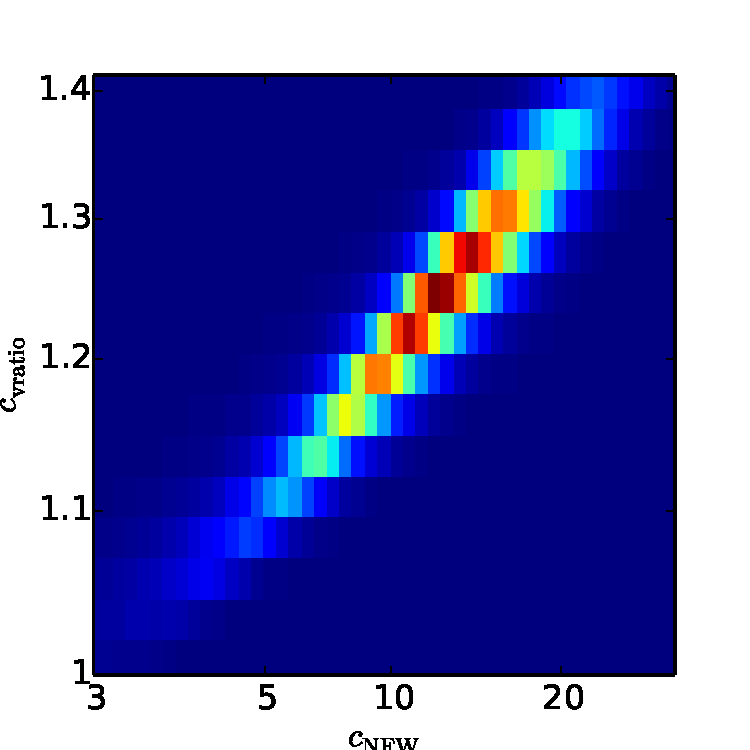
\includegraphics[width=.5\textwidth]{ldcompare_cnfwvscvrat_z00.pdf}
	\caption{The relationship between the two different marks of concentration, using halos in the Consuelo simulation box.}
\end{figure}

%% this does need to be changed over to a rerun on a Diemer simulation box, but that should be fairly quick to do. Just have to find my pipeline code for that and tweak a few things

The first two marks listed above are different proxies for the concentration of the halo. The relationships between these marks are shown in Figure 1 and it can be seen that they can be related to each other with some scatter. The ROCKSTAR catalogs give us the max  circular velocity of a hypothetical particle, $v_{\mathrm{max}}$, the scale radius, $r_{\mathrm{s}}$, the halo radius, $\Rdel$, both ellipsoidal axis parameters $c$ and $a$, and the spin parameter, $\Lambda$ as introduced by \citep{peebles69} in terms of the halo angular momentrum $J$ and the total energy of the halo $E$ . The circular velocity of a particle at the halo radius is calculated by $v_{\Delta} = \sqrt{\frac{G M(< \Rdel)}{\Rdel}}$.

%-----------------------
\section[]{Methodology}
\label{section:methodology}
%-----------------------

There are several well understood effects in our simulation that must be accounted for before we can draw any conclusions. The first is the matter of simulation resolution. In each of our generated halo catalogs, we can anticipate finding artificial halos. While existing under our constraint of having only a set overdensity, they will have properties that conflict with well known trends that have been shown in prior works, such as concentration decreasing as a function of halo mass \citep{wechsler06}. As shown in Figure 2, we can roughly identify the region in which these artificial halos become significant by looking for the turnover in the plot. In order to avoid our halo finding statistics being thrown off by these artificial halos, we set a lower mass threshold, limiting the sample to only those halos that are physically significant. We have chosen our threshold to be set by the L0250 Diemer box in order to minimize the shift to the remaining catalogs.

\begin{figure}
	\centering
		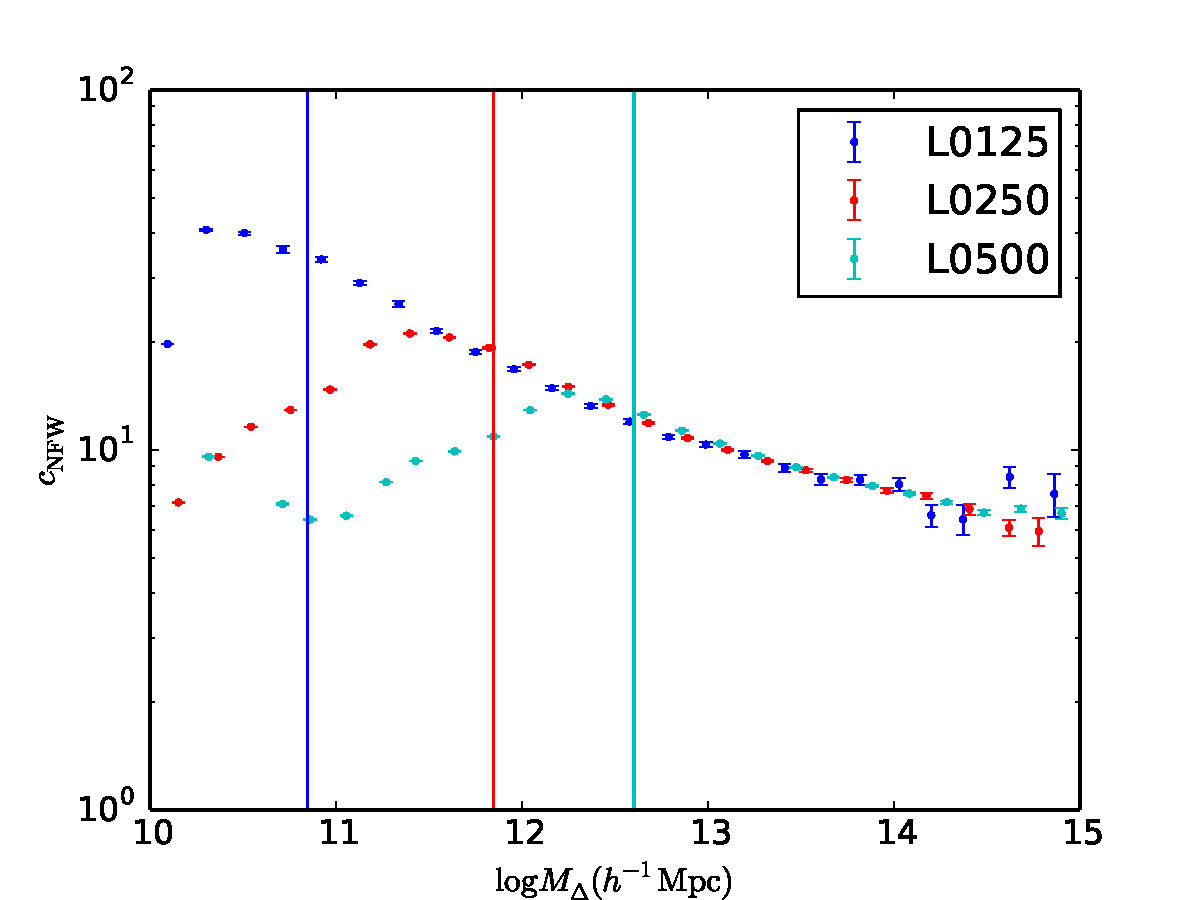
\includegraphics[width=.5\textwidth]{masscut_cnfw_d200.pdf}
	\caption{An example of the chosen lower limit on halo mass for our sample is marked as a black line, for the $\Delta = 200$ case. The shaded blue region depicts the spread on the power in the concentration-mass relationship proposed by \citet{duffy08}.  The shaded region illustrates the implied two-sigma band of \citet{duffy08} mass-concentration relation. At lower mass, halos are ill defined due to resolution limits. \arz{This caption needs to be more specific. Lower limit for which simulation? It looks like maybe for L0250? We should put our lower limits for each simulation. Also, because c(M) is thought to be nearly a power law, the y-axis should be logarithmic as well. Try that and let's see what it looks like.}}
\end{figure}

%% again, this will need to be remade and drop the Consuelo data, but should be quick enough.

Another well known effect is the scaling of our properties as a function of halo mass, as well demonstrated within the literature \citep{duffy08}. We are interested in the clustering behavior beyond this well known effect, so we seek to remove this scaling. We take all host halos of interest and sort them by their halo mass. Each set of halo properties are then placed in bins of equal population in order to assure that enough data points exist for robust statistics. We then normalize each mark in a given bin to the mean value. The end result is halo properties that do not change as a function of mass, allowing us to more accurately analyze clustering behavior within our simulation.

To normalize the satellite number we follow the prescription of \citet{wechsler06}. In addition to the mass cutoffs on our data, we eliminate ill-resolved satellites by choosing a cutoff in $v_{\mathrm{max}}$ for the host halo. We then attempt to match subhalos to this mass halo, making a secondary cutoff in the case that the value of $v_{\mathrm{max,sub}} / v_{\mathrm{max,host}}$ is not above a threshold value. We set these two parameters such that there are no isolated or poorly resolved subhalos in our data sample.

In order to test for environmental effects, we choose to utilize two primary methods. The first is to look at the two-point correlation functions of the host halo catalog and compare it against the correlation functions of the top and bottom 20\% of most concentrated host halos. Assuming that each halo was statistically similar, we would expect that there would be no discernible difference between these correlation functions in the case where there are no environmental effects.

The second method is to use a weighted correlation function, often referred to in the literature as the marked correlation function (MCF). Our marks in this case are the log values of the halo concentration proxies described previously, the halo shape, and the halo satellite number. The use of this tool in measuring clustering has been shown previously in \citet{wechsler06} or \citet{harker06}. We compare our MCFs to an error bar representing the approximate 2-sigma confidence region generated by randomizing the marks among our halos 400 times and taking the 10th lowest and 390th highest values of the mark among the randomizations. In the case of no environmental effects upon the property of interest, one would expect that the MCF would fall within the region bounded by these limits.

%----------------------------
\section[]{Results and Discussion}
\label{section:results}
%----------------------------

Ultimately, as a result of the limited nature of simulation data, we must make some lower mass cutoff in our study of halo properties. Table 1 describes where we have chosen to place these cuts in a variety of different measures. The ``hosts" set of cuts has been chosen for our primary form of analysis, as it it performs well across all four halo boxes. Figure 2 shows the example of this cutoff in the $\Delta = 200$ case. While there may be some concern about the number of low mass halos included in the L0500 simulation box, results seem to demonstrate that the effect is somewhat minimal compared to other factors. This is quite likely related to our methodology by which we remove the inherent mass dependence, as provided that the ranking of the halos in some mass bin does not significantly change, it should result in the same general trends. The remaining two cuts have been chosen to explore any resolution related effects. The ``l0125'' cuts explore the lowest possible mass cutoff that excludes ill resolved halos in the Diemer et. all simulations, while the ``l0500'' set of cuts represent the mass cutoff chosen to avoid contamination due to resolution effects in our largest simulation box.

\begin{table}[]
\centering
\caption{Chosen mass cuts on the simulation boxes, in units of $\hMsun$. The values of the halo overdensity parameter $\Delta$ chosen are listed in the first row.}
\label{my-label}
\begin{tabular}{l | l | l | l | l}
           & 200  & 100  & 75   & 50     \\ \hline
"hosts"    & 7E11 & 8E11 & 9E11 & 1.5E12 \\
"l0125cut" & 7E10 & 8E10 & 9E10 & 1E11   \\
"l0500cut" & 4E12 & 5E12 & 6E12 & 7E12  
\end{tabular}
\end{table}

\begin{figure*}
	\centering
	\subfloat[L0125]{{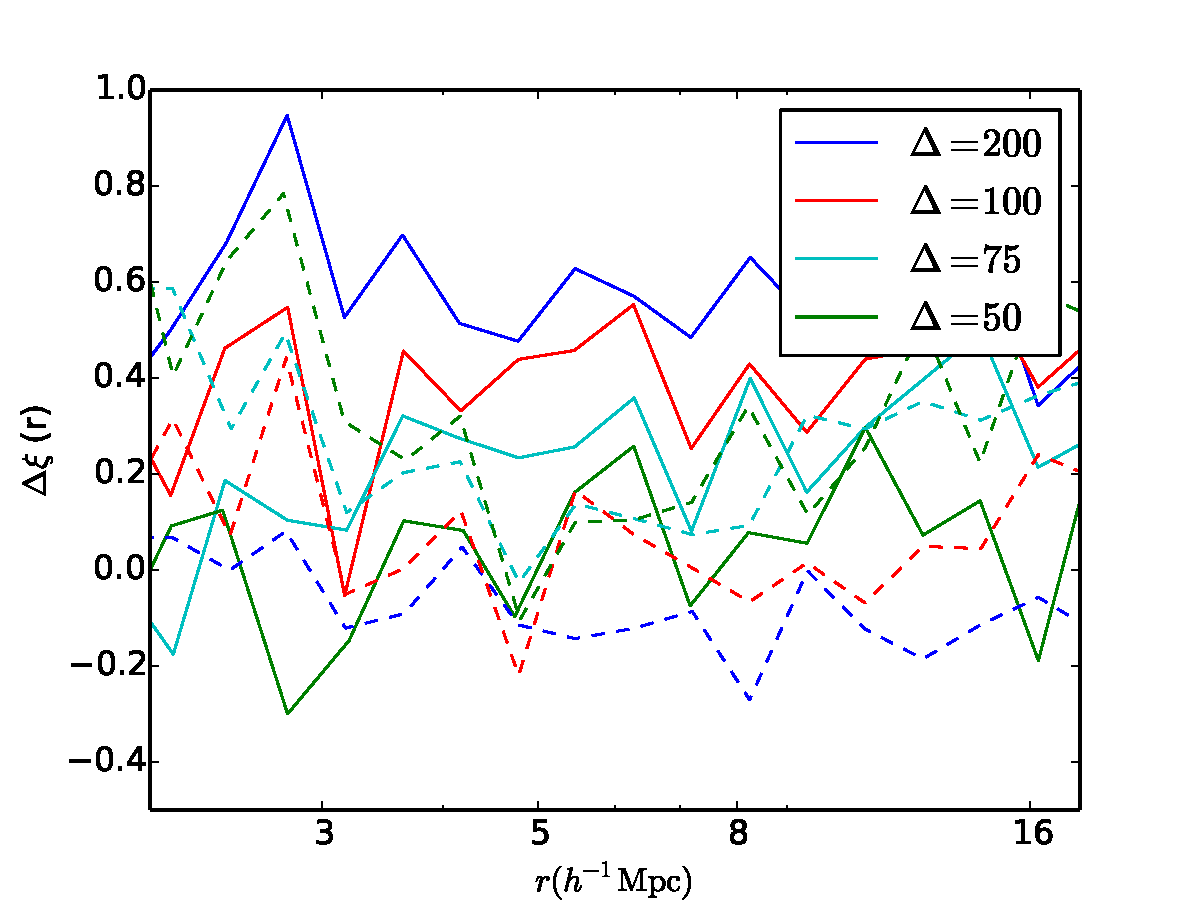
\includegraphics[width=.45\textwidth]{L0125_cf_compare_z00_hosts.pdf}} }
	\subfloat[L0250]{{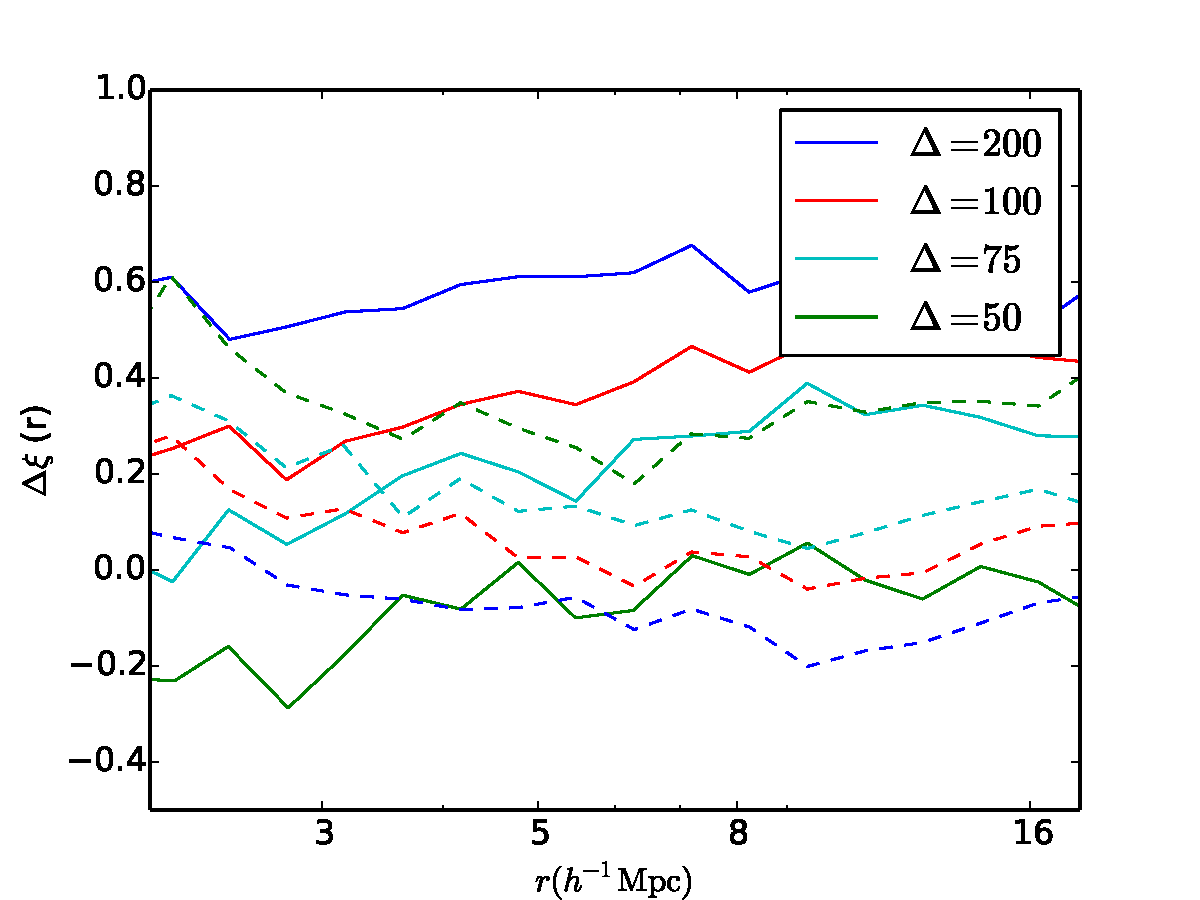
\includegraphics[width=.45\textwidth]{L0250_cf_compare_z00_hosts.pdf}} }
	\\
	\subfloat[L0500]{{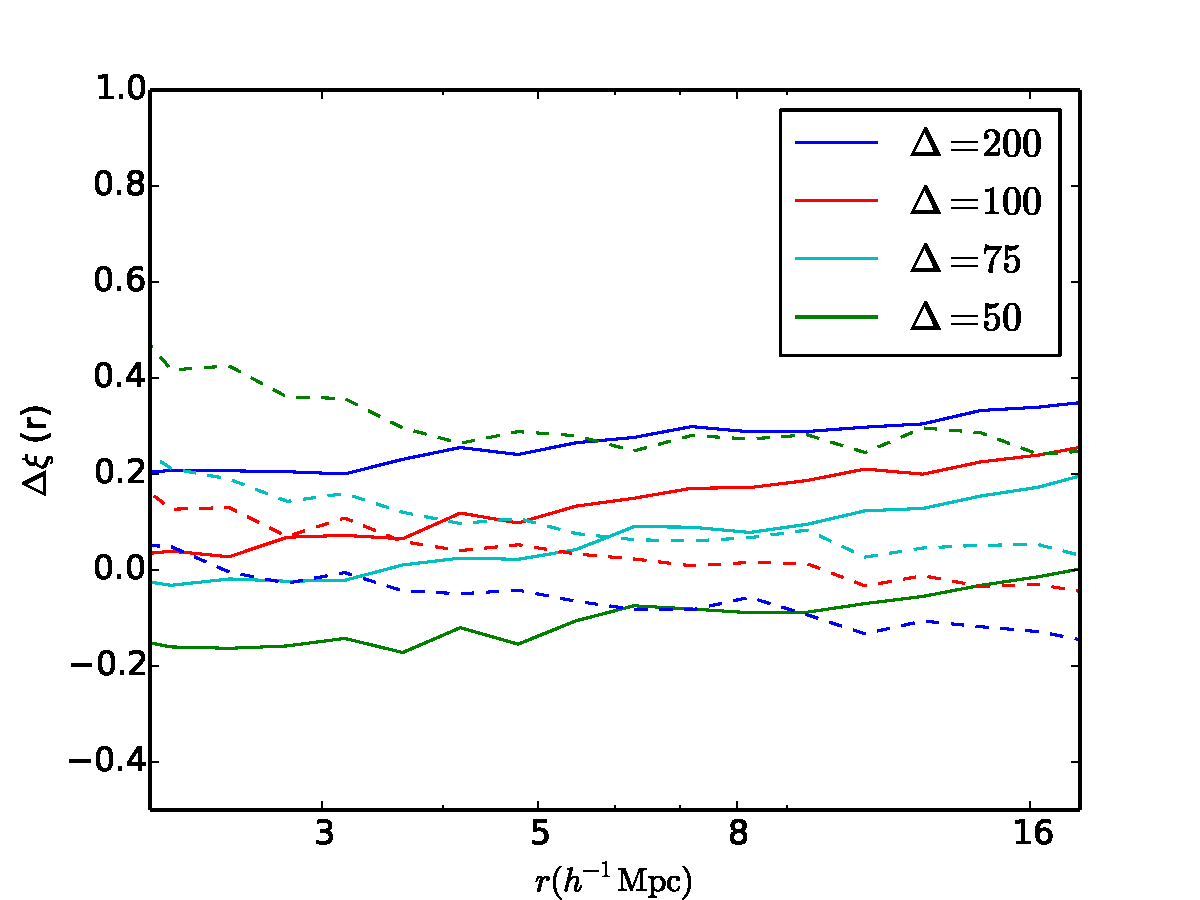
\includegraphics[width=.45\textwidth]{L0500_cf_compare_z00_hosts.pdf}} }
	\subfloat[Consuelo]{{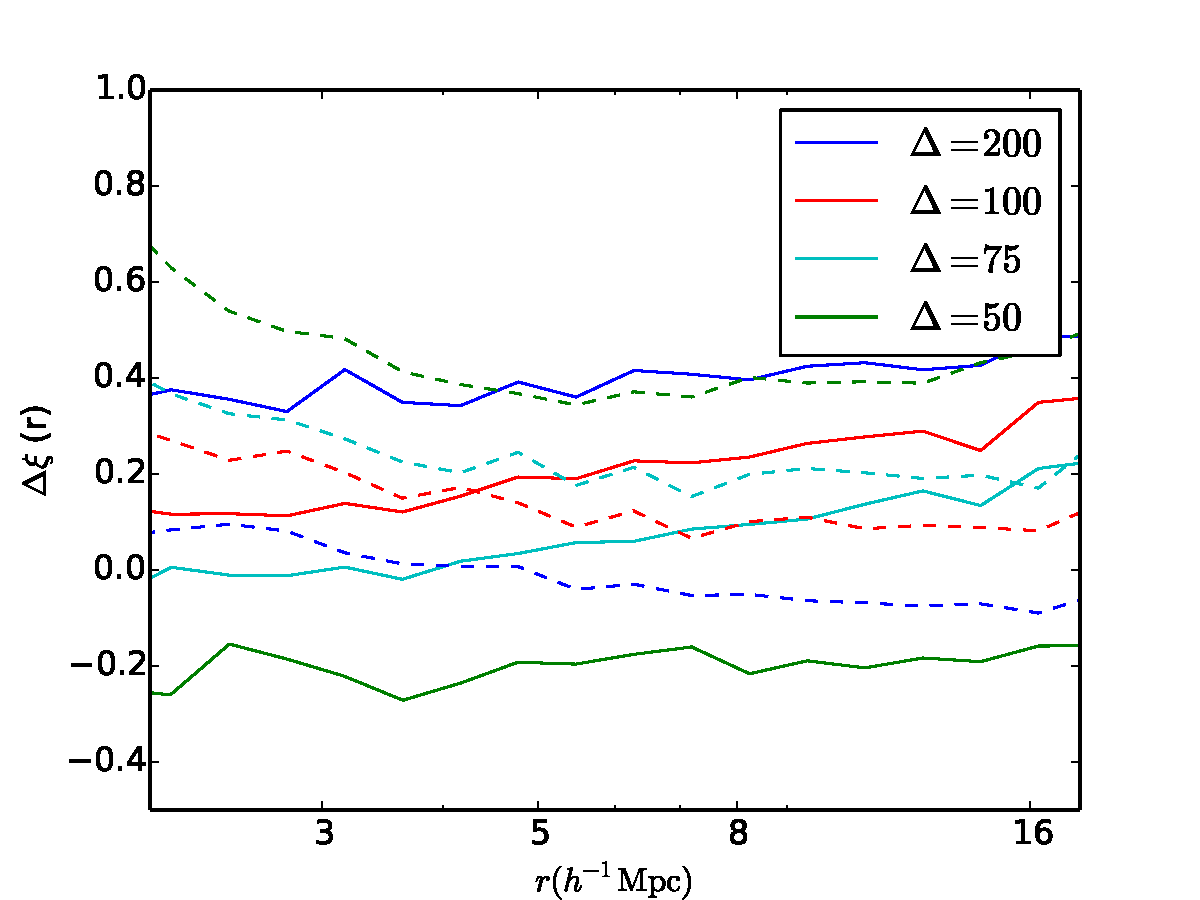
\includegraphics[width=.45\textwidth]{ld_cf_compare_z00_hosts.pdf}} }
	\caption{The difference of the correlation function of all hosts compared to a cut of the 20 \% highest or lowest NFW defined concentration halos. The solid lines represent the difference from the highest concentration cut, the dashed lines represent the difference from the lowest concentration cut. \arz{We'll have to think carefully about this figure. It is very hard to read. Perhaps we can show just Delta=200 and then your "best" Delta? Also, we can remove the Consuelo reference.}}
\end{figure*}

%% this plot also escaped my workflow. I'll add it to the main plot generator.

The left column of Figure 3 demonstrates the results of our method as we change the value of $\Delta$. It can be seen that for between the values of $\Delta = 75$ and $\Delta = 50$ that both the high and low concentration cuts of the data can be brought into close agreement in the Diemer et. al boxes. It should be noted that both the high and low concentration cuts move closer toward a state with environmental dependencies being thoroughly removed within the margin of error from opposite directions in terms of clustering. Changing the value of $\Delta$ beyond the observed ``sweet spot" appears to reintroduce the problem we are attempting to remove.

\begin{figure*}
	\centering
	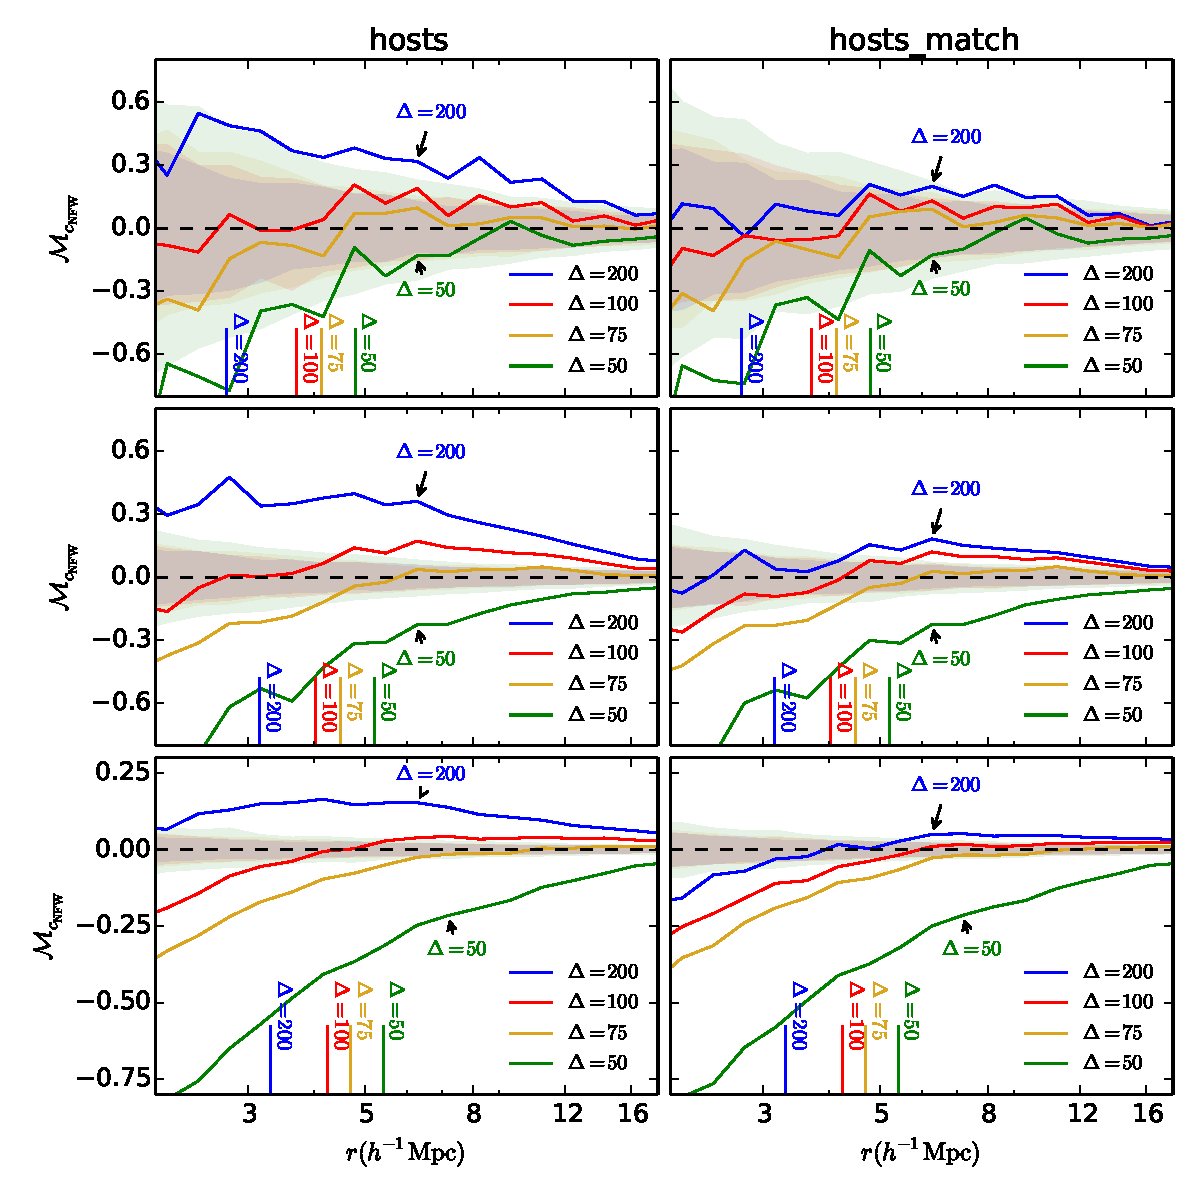
\includegraphics[width=\textwidth]{all_mcf_cnfw_z00_hostsvmatch.pdf}
	\caption{The marked correlation function for the concentration defined according to the NFW profile. From top to bottom, we show the results for the Diemer L0125, L0250, and L0500 boxes. The left column utilizes all host halos in the catalog. The right column contains only host halos that exist inside of our best fit value of $\Delta$, as explained in the text. The shaded bands represent 2-sigma confidence regions generated by randomization of the marks. The dashed line denotes the largest halo radius for a given value of the overdensity parameter. \arz{This figure is beautiful now. The only recommendation I have is to remove the white space in the lowest row of panels. Perhaps make the maximum y-axis 0.25 or so.}}
\end{figure*}

The NFW defined concentration MCF is shown in the left column of Figure 4. It can been that as we decrease the value of the overdensity parameter $\Delta$ to lower values down to $\Delta = 50$. It can be seen that at scales of $r > 10 \hMpc$, environmental effects are removed between $\Delta = 75$ and $\Delta = 50$ in the Diemer et al. boxes. This is repeated for the velocity ratio defined concentration in the left column of Figure 5. It again demonstrates that the same values of $\Delta$ are preferred for the removal of assembly bias as with the NFW concentration. This seems to indicate that our methodology should be effective at minimizing the impact of assembly bias at large scales.

\begin{figure*}
	\centering
	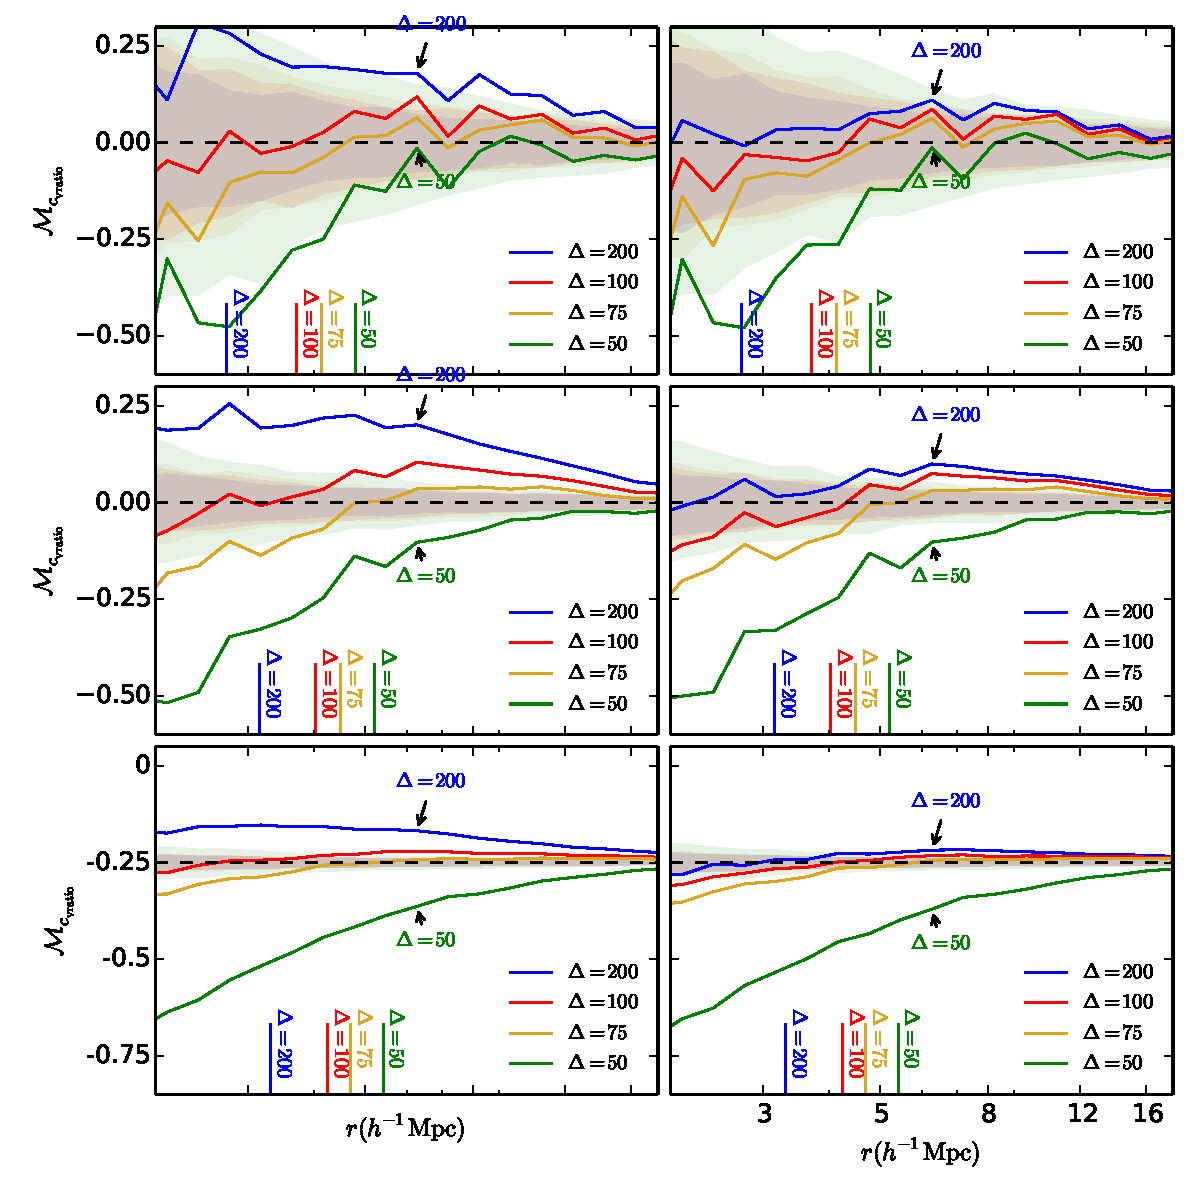
\includegraphics[width=\textwidth]{all_mcf_cvratio_z00_hostsvmatch.pdf}
	\caption{The marked correlation function for the concentration defined according to the velocity ratio. From top to bottom, we show the results for the Diemer L0125, L0250, and L0500 boxes. The left column utilizes all host halos in the catalog. The right column contains only host halos that exist inside of our best fit value of $\Delta$, as explained in the text. The shaded bands represent 2-sigma confidence regions generated by randomization of the marks. The dashed line denotes the largest halo radius for a given value of the overdensity parameter. \arz{This figure needs to be made as beautiful as Figure 4.}}
\end{figure*}

\begin{figure*}
	\centering
	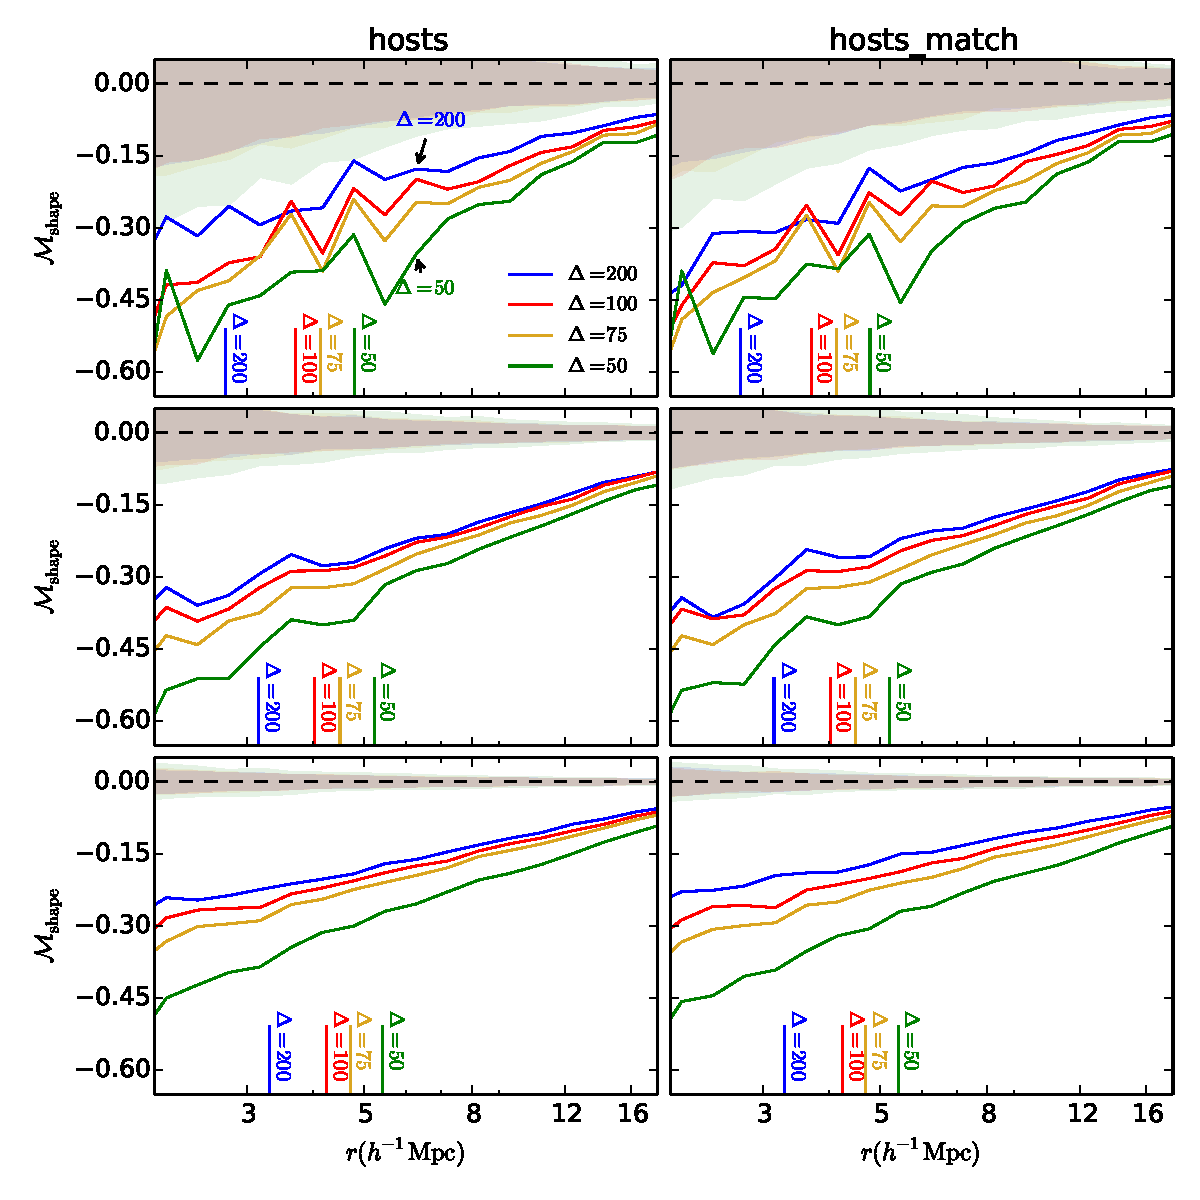
\includegraphics[width=\textwidth]{all_mcf_s_z00_hostsvmatch.pdf}
	\caption{The marked correlation function for the shape of the halo. From top to bottom, we show the results for the Diemer L0125, L0250, and L0500 boxes. The left column utilizes all host halos in the catalog. The right column contains only host halos that exist inside of our best fit value of $\Delta$, as explained in the text. The shaded bands represent 2-sigma confidence regions generated by randomization of the marks. The dashed line denotes the largest halo radius for a given value of the overdensity parameter.}
\end{figure*}

The left column of Figure 6 demonstrates a case in which the halo property does not have environmental dependence removed under our simple method of halo redefinition. In particular, with decreasing values of $\Delta$, we only serve to increase the strength of this environmental dependence. This result seems to indicate a process occurring to drive the shape of the halo is on scales that are significantly larger than the size of the halo, such that our method will not be able to encompass these effects. A similar result is located in both the left columns of Figure 7 and Figure 8, in which the spin parameter mark and satellite number mark experience the exact same effect.

\begin{figure*}
	\centering
	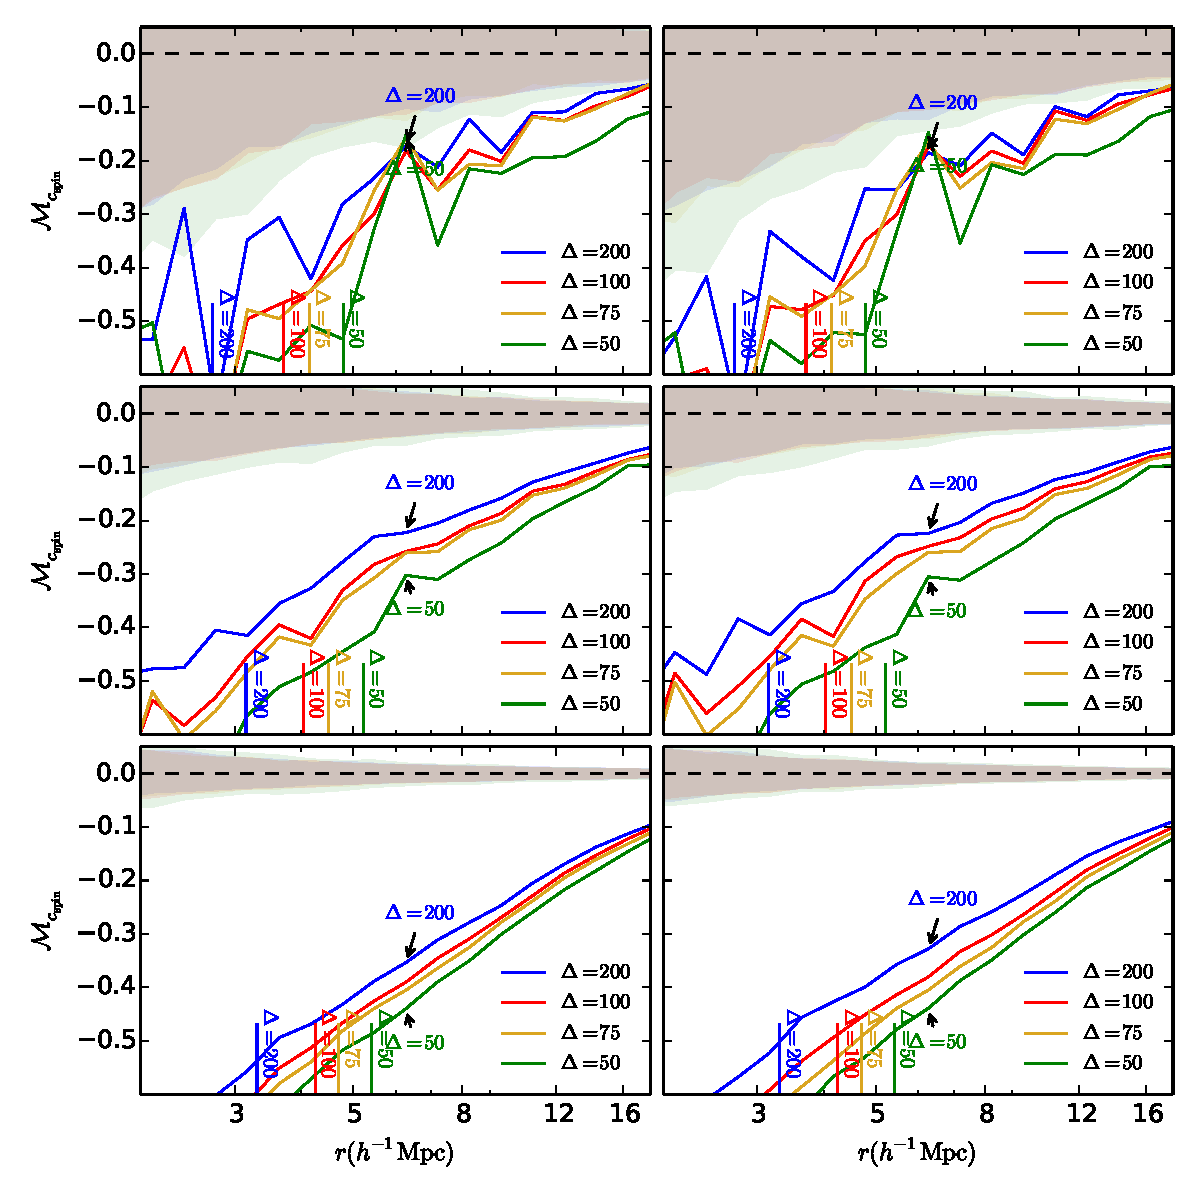
\includegraphics[width=\textwidth]{all_mcf_spin_z00_hostsvmatch.pdf}
	\caption{The marked correlation function for the spin parameter of the halo. From top to bottom, we show the results for the Diemer L0125, L0250, and L0500 boxes. The left column utilizes all host halos in the catalog. The right column contains only host halos that exist inside of our best fit value of $\Delta$, as explained in the text. The shaded bands represent 2-sigma confidence regions generated by randomization of the marks. The dashed line denotes the largest halo radius for a given value of the overdensity parameter.}
\end{figure*}

\begin{figure*}
	\centering
	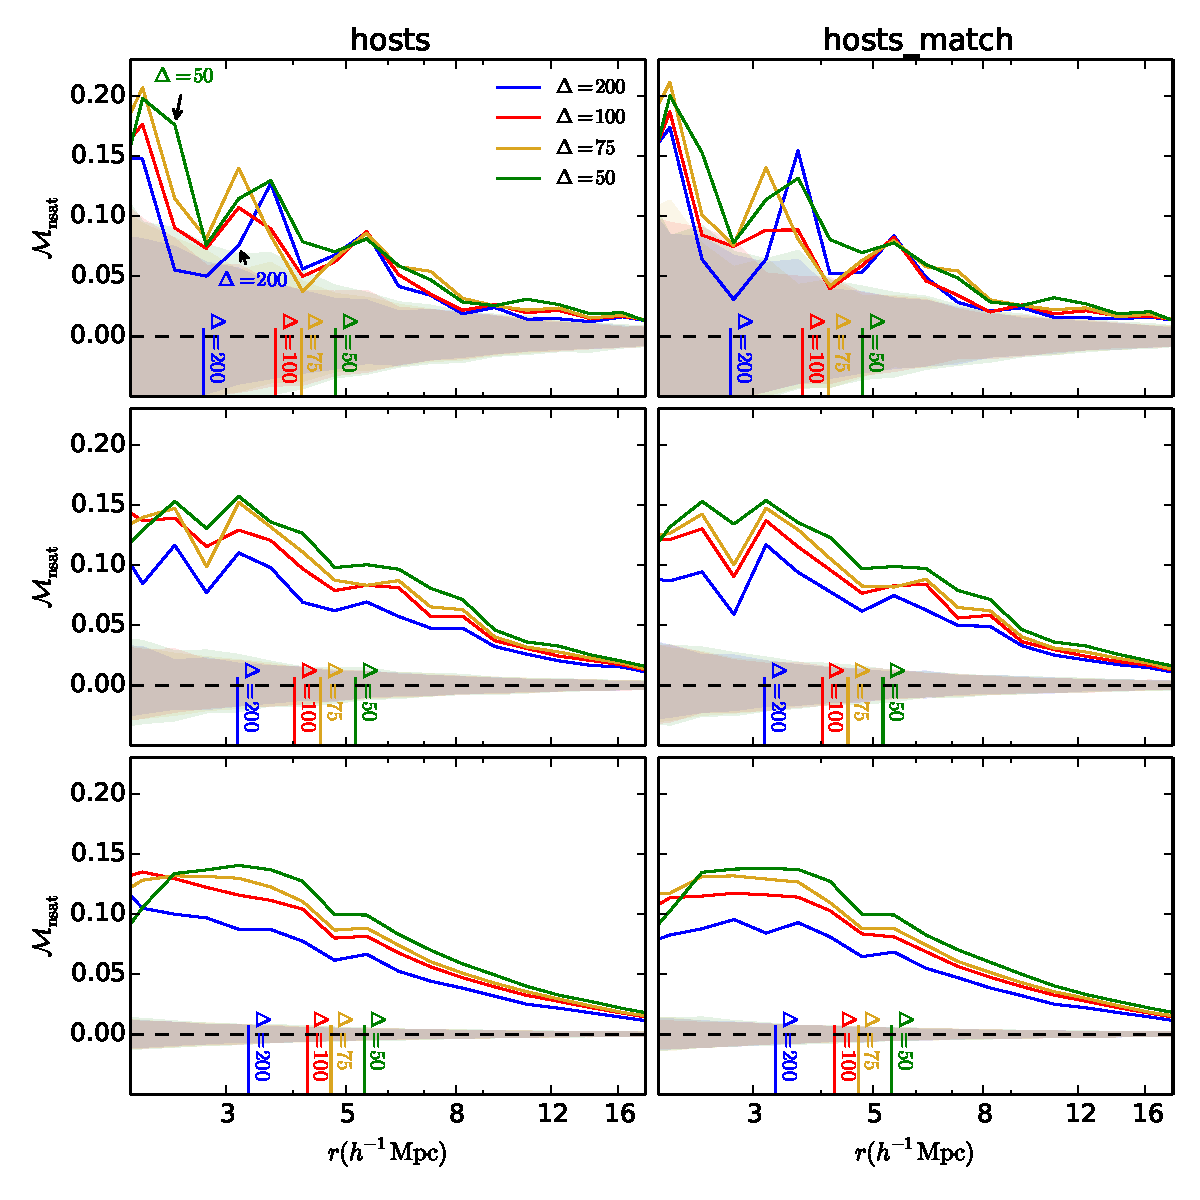
\includegraphics[width=\textwidth]{all_mcf_nsat_z00_hostsvmatch.pdf}
	\caption{The marked correlation function for the number of satellites for a host halo. From top to bottom, we show the results for the Diemer L0125, L0250, and L0500 boxes. The left column utilizes all host halos in the catalog. The right column contains only host halos that exist inside of our best fit value of $\Delta$, as explained in the text. The shaded bands represent 2-sigma confidence regions generated by randomization of the marks. The dashed line denotes the largest halo radius for a given value of the overdensity parameter.}
\end{figure*}

Overall, while some statistics of the halo can be made to become independent of environmental effects, there exist several that cannot. These environmental effects are not negligible when considering applications of the halo model. In contrast, if one is only interested in the concentration of the halo, it is feasible to take advantage of our methodology in order to remove environmental effects. In contrast, it is not possible to apply the halo model directly to statistics such as the number of satellite halos or the shape without accounting for these environmental effects. We do not yet have a full understanding of what leads to the visible effects that we see on some of these marks, but we present a series of cases in which an intuitive understanding may be gained as to the root causes.

We would also like to study our sample for some insight as to how this process of correction is actually functioning. For example, we would like to know if it is a more careful selection of halos in our simulation that results in the removal of this apparent assembly bias or if it is the increased noise in the statistics as a result of reducing the number of halos. There is also the possibility of halo statistics changing as a result of the new halo definitions to be considered. One can imagine that the addition of a large amount of mass toward the edge of the halo would reasonably change measures of concentration, shape, and spin. To test some of these possibilities, we run an algorithm to match halos across our multiple catalogs. We identify halos that are within a distance tolerance that we scale such that there are no identifications of multiple halos to the same object in another catalog. Catalogs are all matched against a single target catalog. This target catalog is chosen to fit the value of $\Delta$ that we find best removes assembly bias in large scales for the concentration marks chosen. For the Diemer et al. simulations, we find this to be a value of approximately $\Delta = 70$. Once the catalogs have been matched against this primary catalog, we rerun our marked correlation function calculations using only host halos identified across both catalogs. This tests if the exclusion of halos that are subsumed in the lower $\Delta$ catalog is the primary cause of our results as well as those halos that are commonly referred to as backsplash halos.

We can see the results of this test in Figures 3 through 8. Comparing in each case, the $\Delta = 200$ result when utilizing a catalog matched to our best fit $\Delta$ demonstrates less assembly bias than the full catalog for the mass cut would demonstrate for our concentration marks. While the magnitude of this result does vary with scale, upwards of 80\% of assembly bias can be accounted for as a result of this selection effect. Furthermore, most of the removed assembly bias occurs on scales that are comparable to the increase in the halo radius between the samples. This seems to indicate that there is significant contamination of host halo statistics by backsplash halos and other halos that would be subsumed into a common host given an increase in halo size.

However, it is worth noting that statistics such as spin parameter, shape, and satellite numbers do not benefit from this selection effect. Assembly bias in these statistics remains nearly identical, suggesting that the selection effects that preferentially account for backsplash halos do not impact these marks. This does serve as a consistency check: given that our methodology does not seem to have a positive impact on the behavior of these marks, the fact that this selection criteria would have positive impact on the data would be an oddity. Instead, we have another confirmation as to the intrinsic ties between these halo statistics and environment.

Given that the removal of assembly bias is not being driven by introducing noice, we now will attempt to determine why the different marks exhibit different behaviors. The first interesting feature is how well our two separate definitions of concentration interact with each other. In the case that the halo can be described well by an NFW profile, one expects a direct relationship between the NFW defined halo concentration and the velocity ratio defined halo concentration. While some variation can be expected due to halos not perfectly being fit by an NFW profile, we do see that the features in one concentration proxy are mirrored in the other. This allows for the two concentration markers to support each other well with regards to our ability to remove environmental effects on large scales.

Halo shape and satellite number are statistics that do not end up having their environmental effects removed and can even be made more prominent by our methodology. One intuitive way to consider the former statistic is in the context of the cosmic web. Studies have shown a statistically significant alignment between filaments and satellite galaxy position \citep{tempel15, velliscig15}. Our method then expands the halo radius and subsumes material that was previously outside of the halo. A simple graphic illustrates this potential effect in Figure 9. As there is a preferential distribution of these satellites that are being subsumed into the halo, this would serve to induce a shape to the halo that would then be determined by Rockstar. In addition, as our satellite number is chosen by those halos within the halo radius, we anticipate that the most clustered regions would see the largest increase in satellite count and thus see an increase in the satellite number mark.

The ``sweet spot'' behavior of this method is also of interest to us. The halo redefinition process that we use serves to decrease halo clustering for the most concentrated halos and increase halo clustering for the least concentrated halos. In the case of the high concentration cut, the reduced clustering can be seen as a result of halo exclusion. As we exchange collections of tightly clustered smaller halos for a single larger halo, then the most prominent contribution of the two-point correlation function will be reduced at all scales.

\begin{figure*}
	\centering
	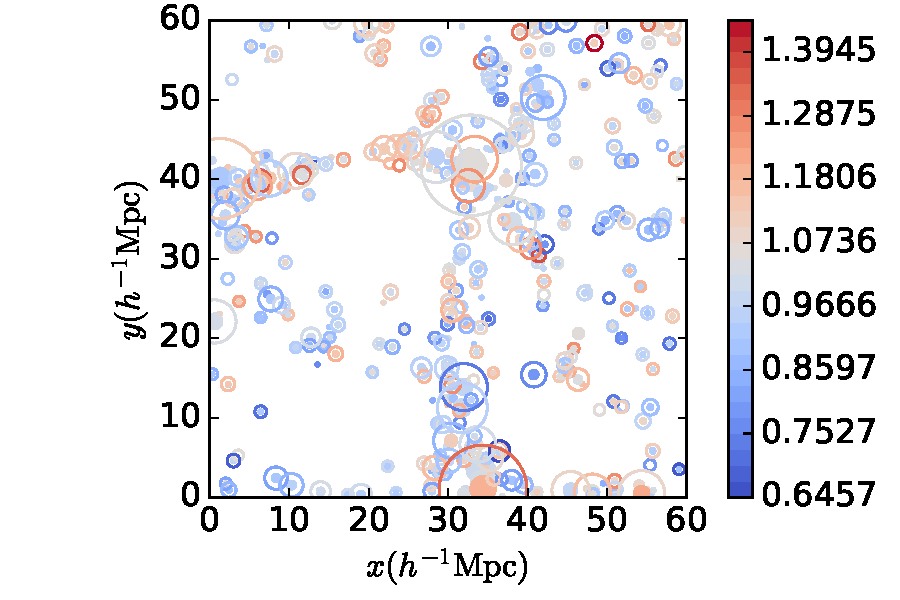
\includegraphics[width=1\textwidth]{plotcircles.pdf}
	\caption{A $5 \hMpc$ deep cut of the Consuelo simulation box along the z-axis. This zoom-in demonstrates the process that decreases the shape parameter as a function of clustering. The size of each circle represents the projection of a spherical dark matter halo with a given halo radius onto the x-y plane. Blue circles use the $\Delta = 200$ catalog and red circles use the $\Delta = 10$ catalog in order to make the effect more visible.}
\end{figure*}

%% another thing to repeat on one of the Diemer boxes. Top priority.

Given the differences between the simulation results and with the data available to us with the Diemer et al. simulations, we then explore the effect of the choice in mass cut. The low mass cut effects are shown in the Figures 10 through 16. This cut explores the area in which we are including ill-resolved halos potentially into the simulation. Namely, utilizing this mass cut on the L0250 simulation box data includes halos that do not fit the form of the expected monotonic halo mass-concentration relation. We can determine several facts from this exercise in resolution testing. The first is that the general behavior of the marks seems to be the same regardless of the influence of the resolution effects. Decreasing the value of $\Delta$ still moves our marked correlation functions in the same directions as the previous mass cut, although often from a very different starting location. A second interesting fact is that despite the L0250 simulation potentially having ill-resolved halos included in the sample, the effect on the overall marked correlation function result is relatively minor. Both samples seem to converge to the same answers within simulation variance. Finally, it should be noted that an unreasonable amount of reduction in $\Delta$ is necessary to bring the lowest mass halos into a region where they will work with this method. We will further explore this effect in the highest mass cuts.

\begin{figure*}
	\centering
	\subfloat[L0125]{{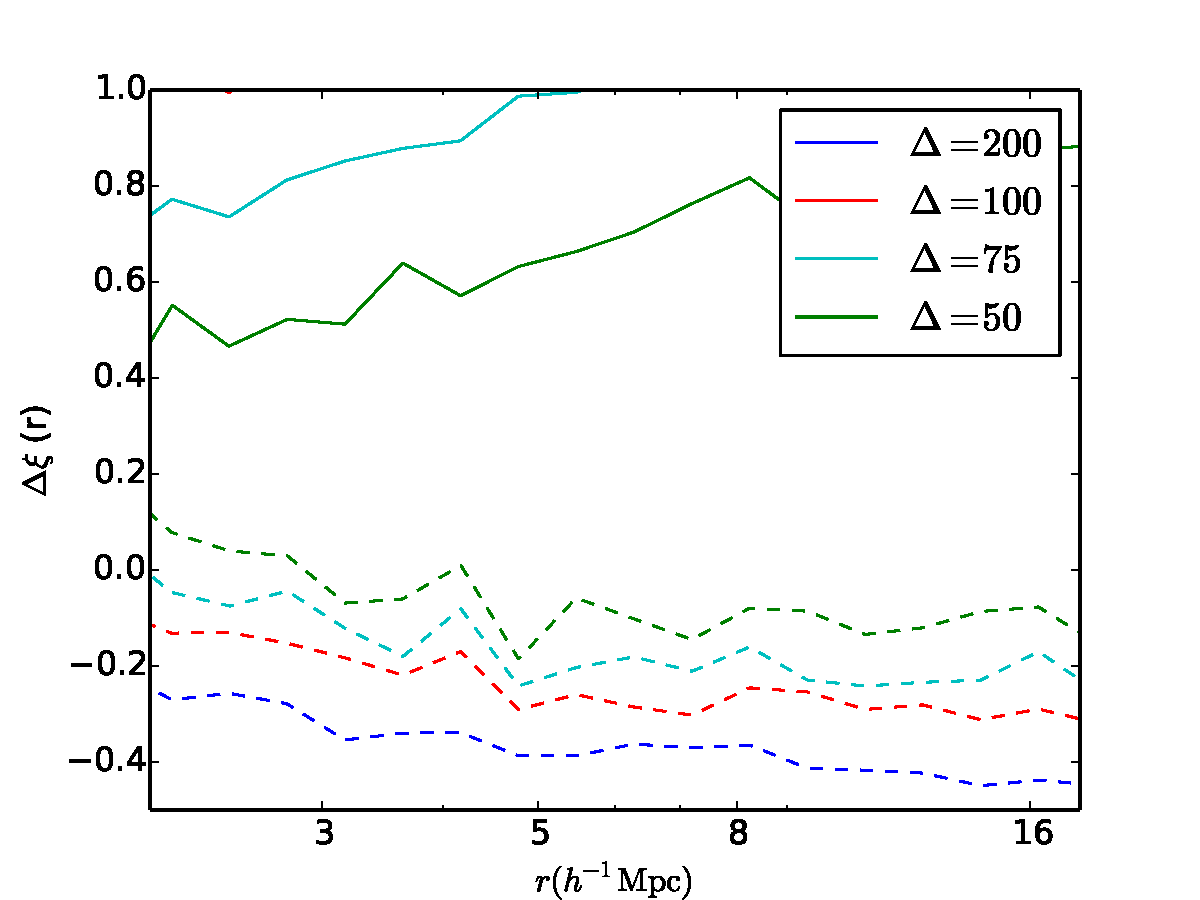
\includegraphics[width=.45\textwidth]{L0125_cf_compare_z00_l0125cut.pdf}} }
	\subfloat[L0250]{{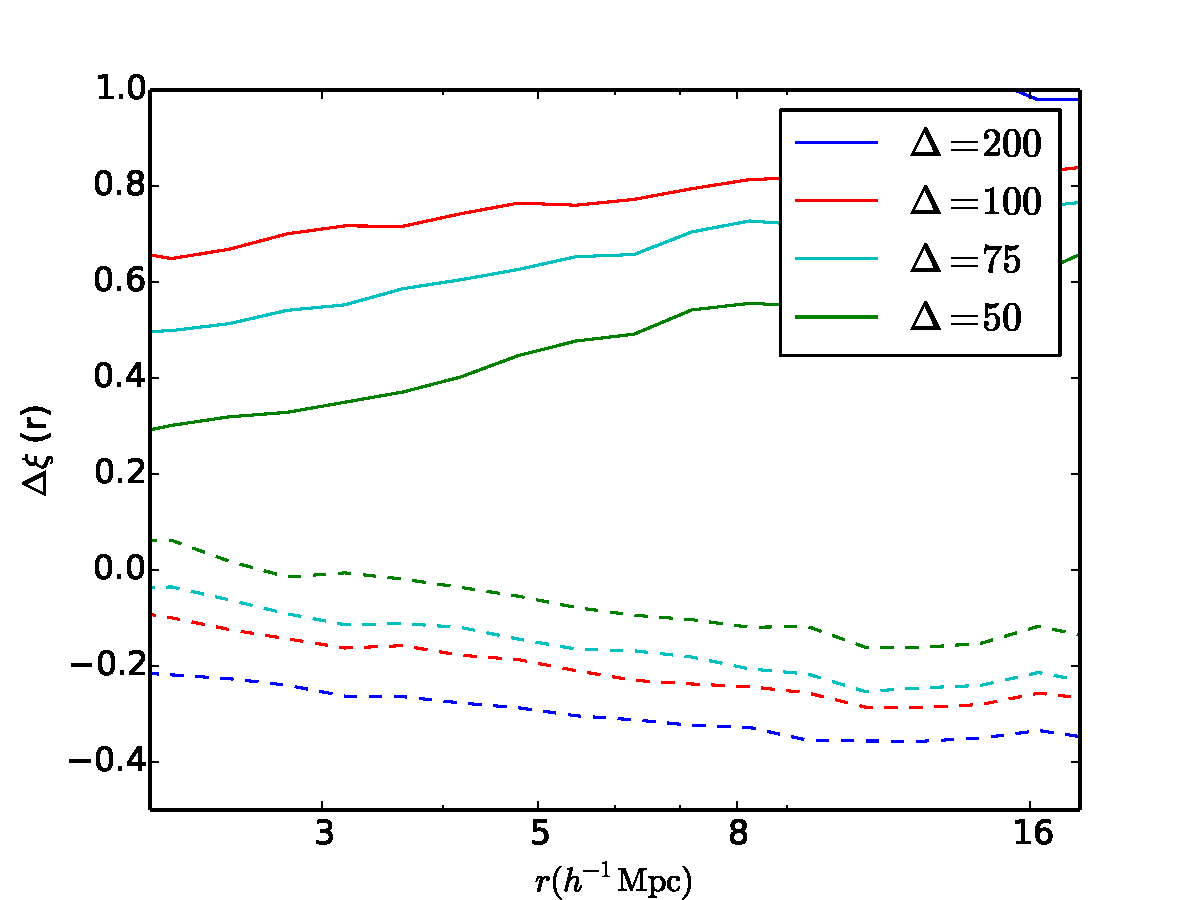
\includegraphics[width=.45\textwidth]{L0250_cf_compare_z00_l0125cut.pdf}} }
	\caption{The difference of the correlation function of all hosts compared to a cut of the 20 \% highest or lowest NFW defined concentration halos utilizing the 'l0125cut' mass cutoffs. The solid lines represent the difference from the highest concentration cut, the dashed lines represent the difference from the lowest concentration cut.}
\end{figure*}

\begin{figure*}
	\centering
	\subfloat[L0125]{{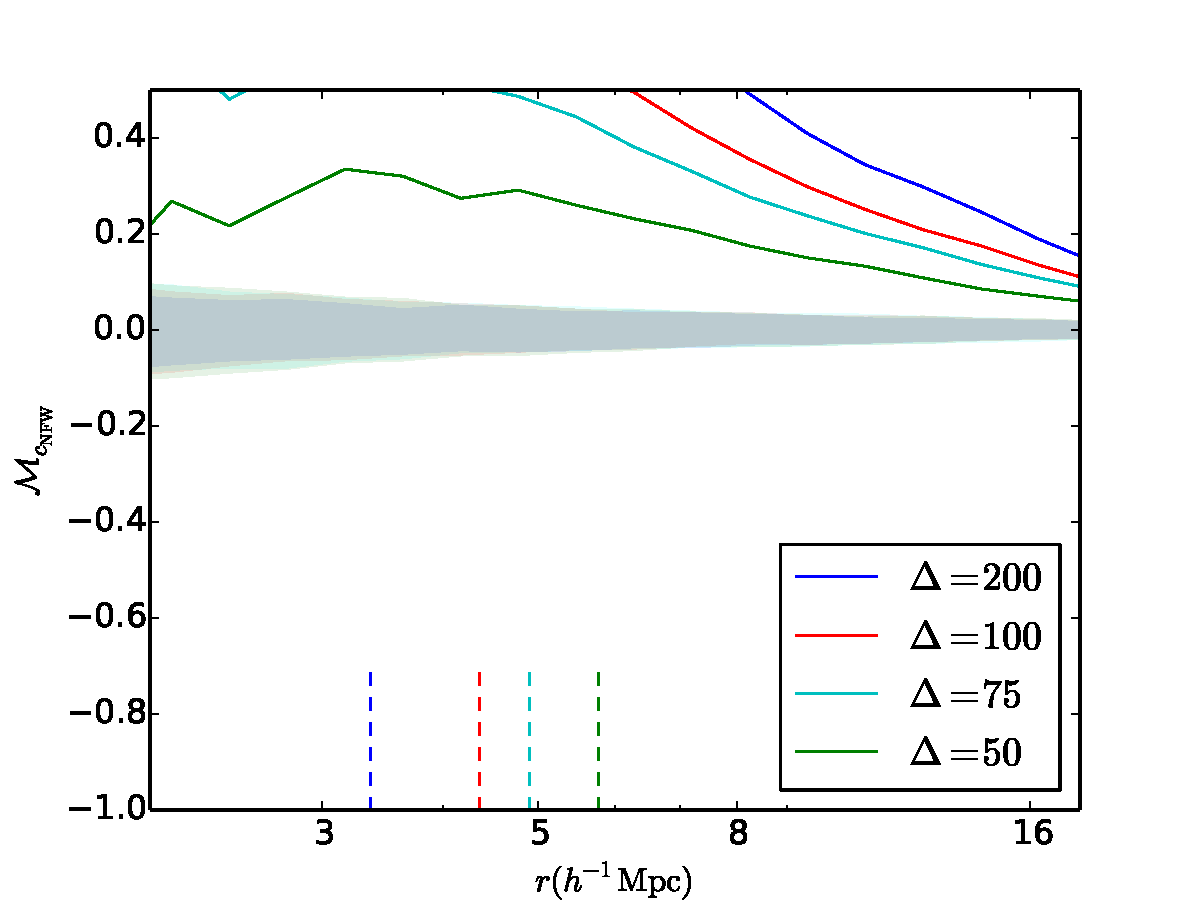
\includegraphics[width=.45\textwidth]{L0125_mcf_cnfw_z00_l0125cut.pdf}} }
	\subfloat[L0250]{{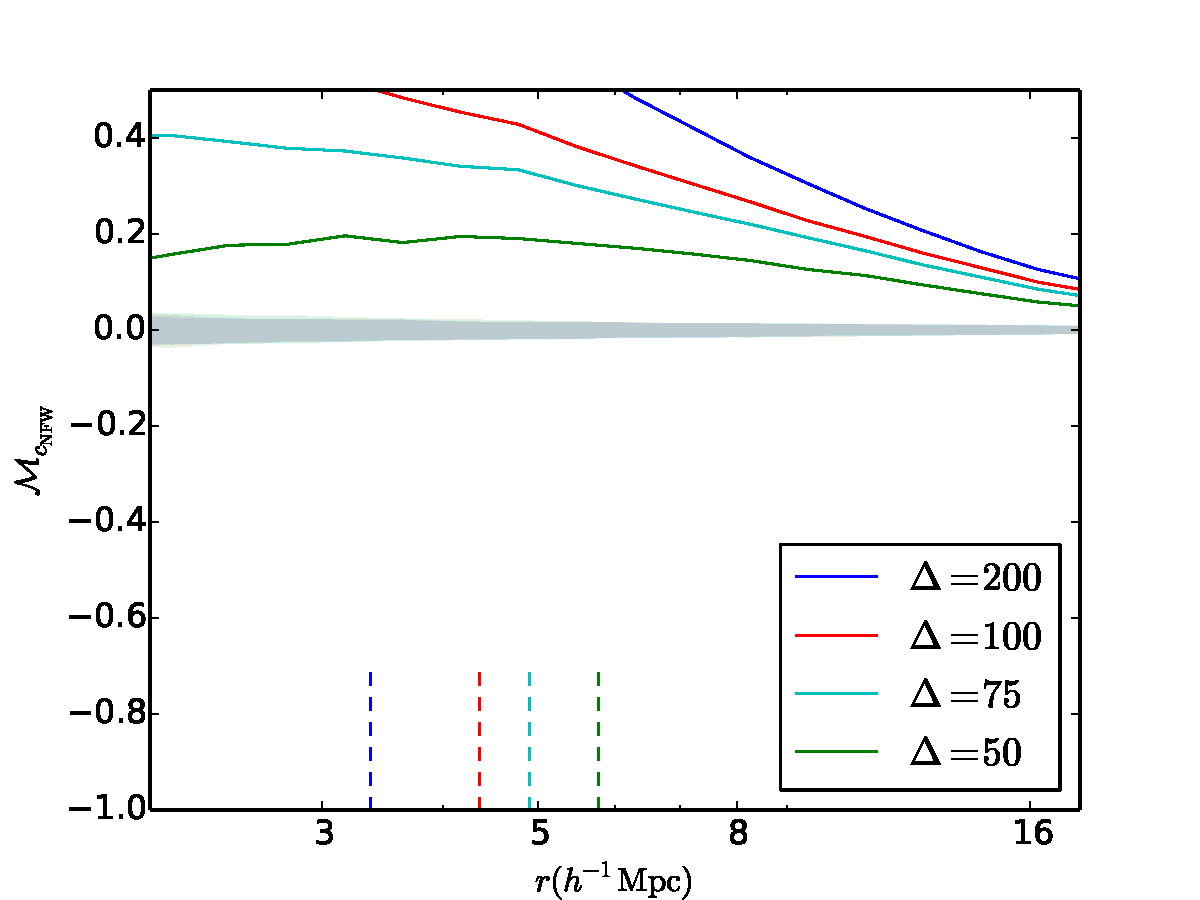
\includegraphics[width=.45\textwidth]{L0250_mcf_cnfw_z00_l0125cut.pdf}} }
	\caption{The marked correlation function for the concentration defined according to the NFW profile utilizing the 'l0125cut' mass cutoffs. The shaded bands represent 2-sigma confidence regions generated by randomization of the marks. The dashed line denotes the largest halo radius for a given value of the overdensity parameter.}
\end{figure*}

\begin{figure*}
	\centering
	\subfloat[L0125]{{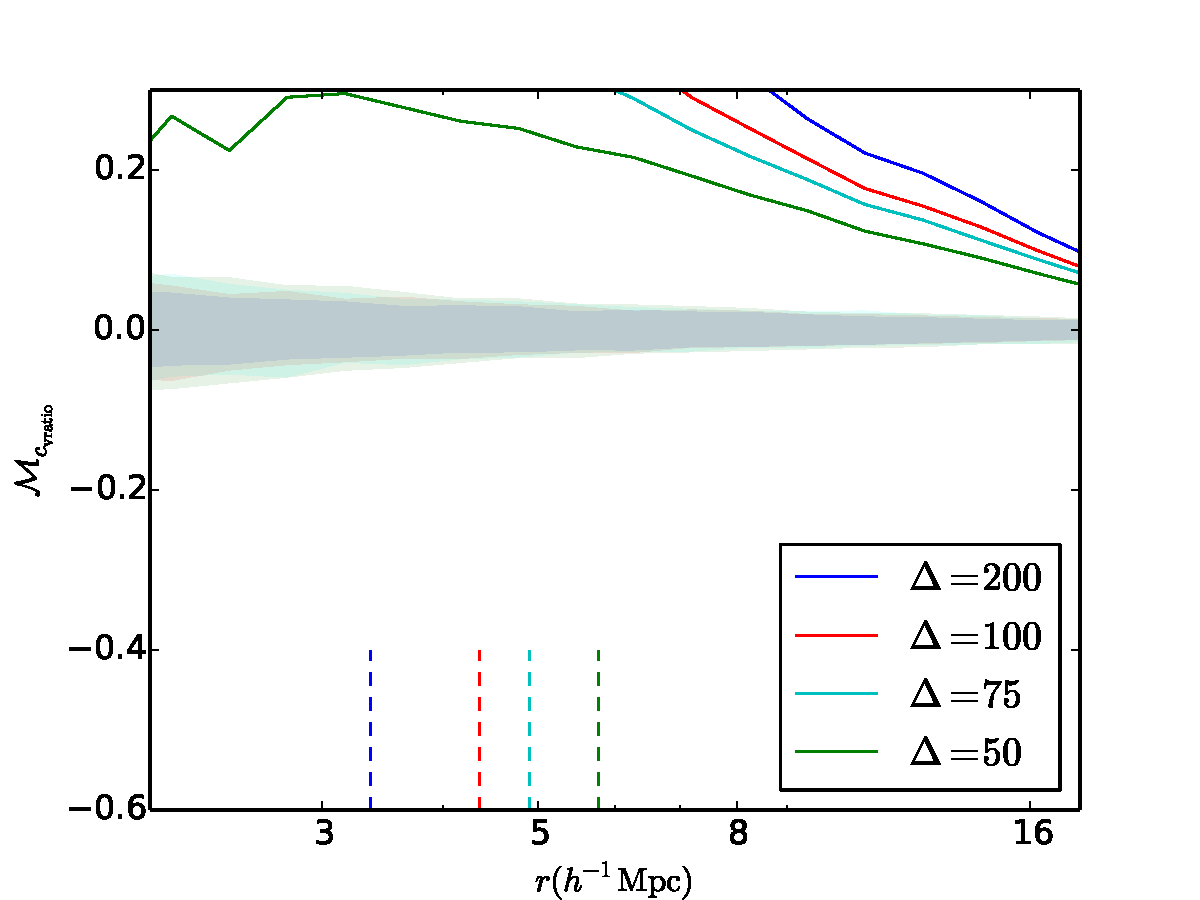
\includegraphics[width=.45\textwidth]{L0125_mcf_vrat_z00_l0125cut.pdf}} }
	\subfloat[L0250]{{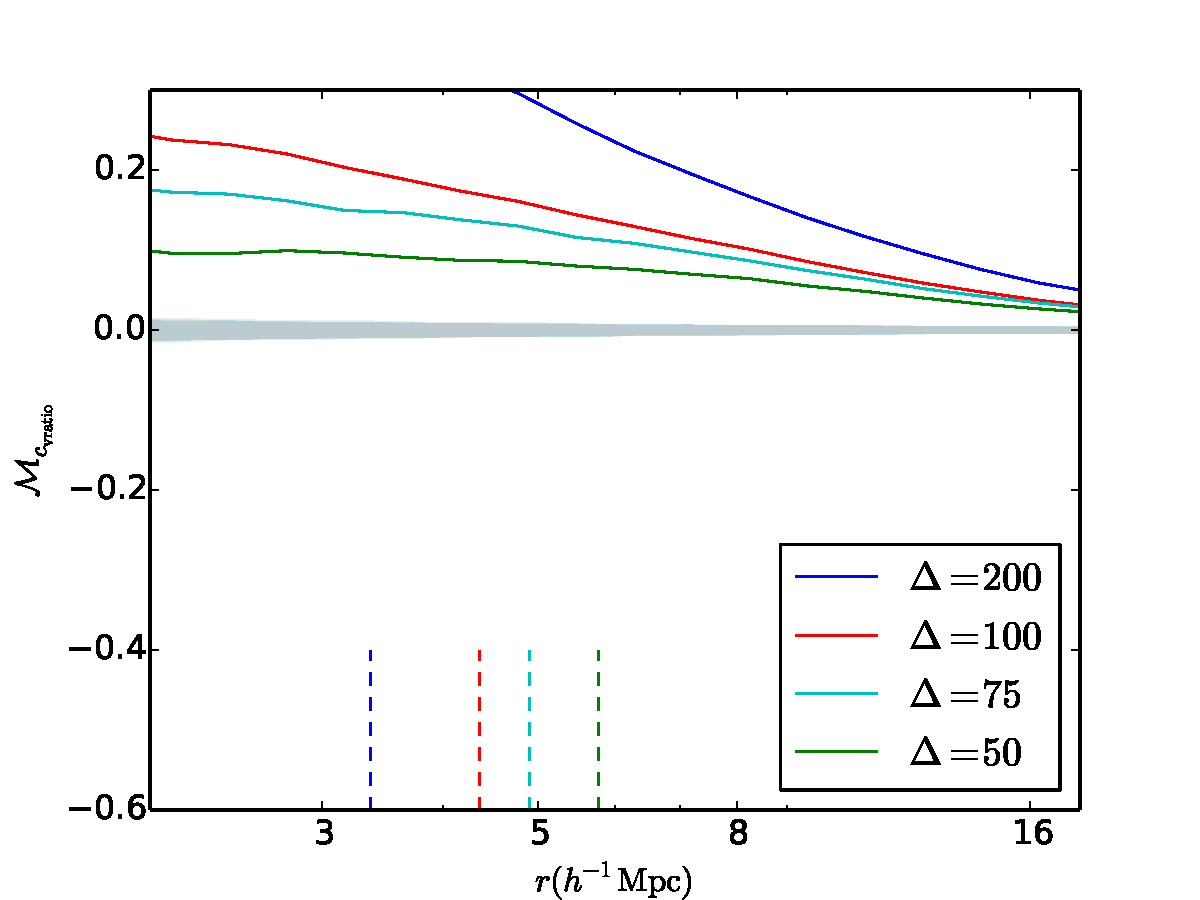
\includegraphics[width=.45\textwidth]{L0250_mcf_vrat_z00_l0125cut.pdf}} }
	\caption{The marked correlation function for the concentration defined according to the velocity ratio utilizing the 'l0125cut' mass cutoffs. The shaded bands represent 2-sigma confidence regions generated by randomization of the marks. The dashed line denotes the largest halo radius for a given value of the overdensity parameter.}
\end{figure*}

\begin{figure*}
	\centering
	\subfloat[L0125]{{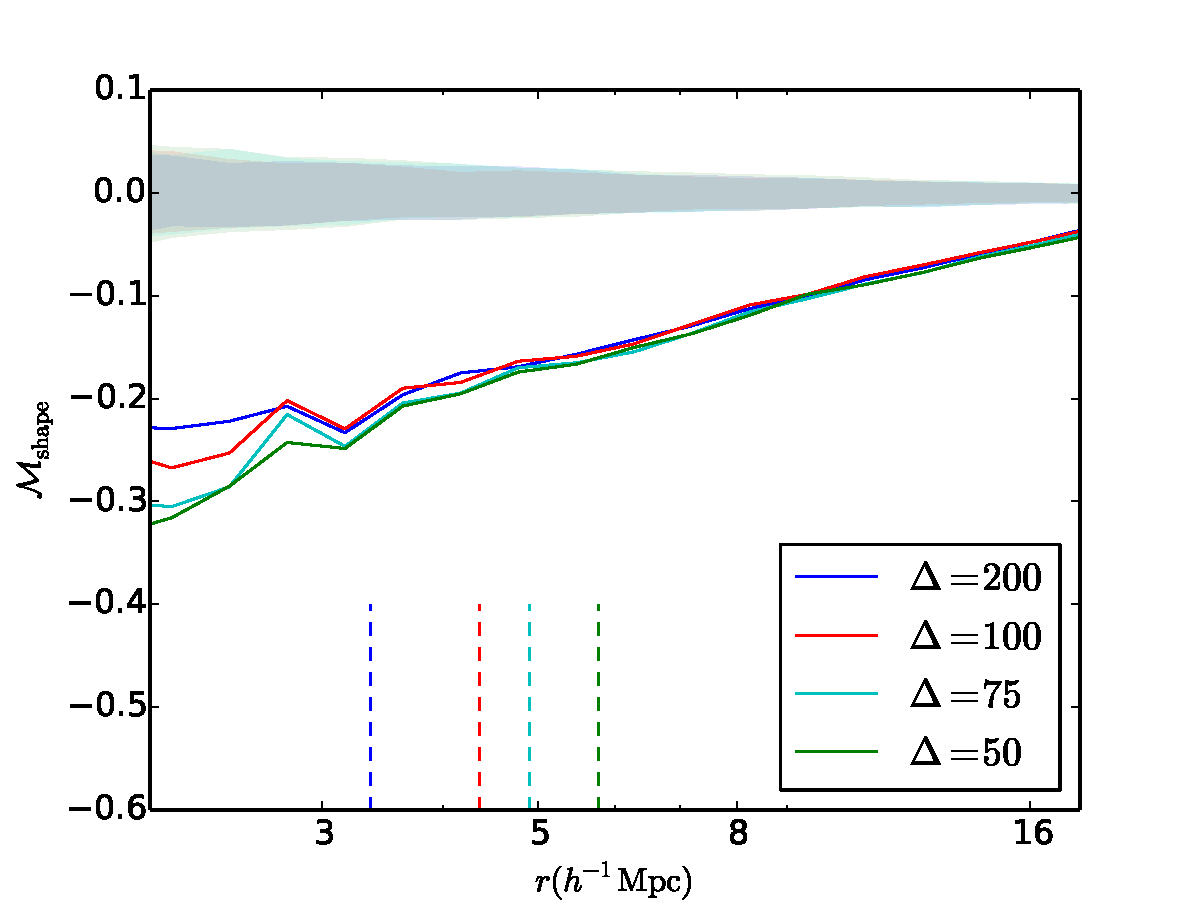
\includegraphics[width=.45\textwidth]{L0125_mcf_s_z00_l0125cut.pdf}} }
	\subfloat[L0250]{{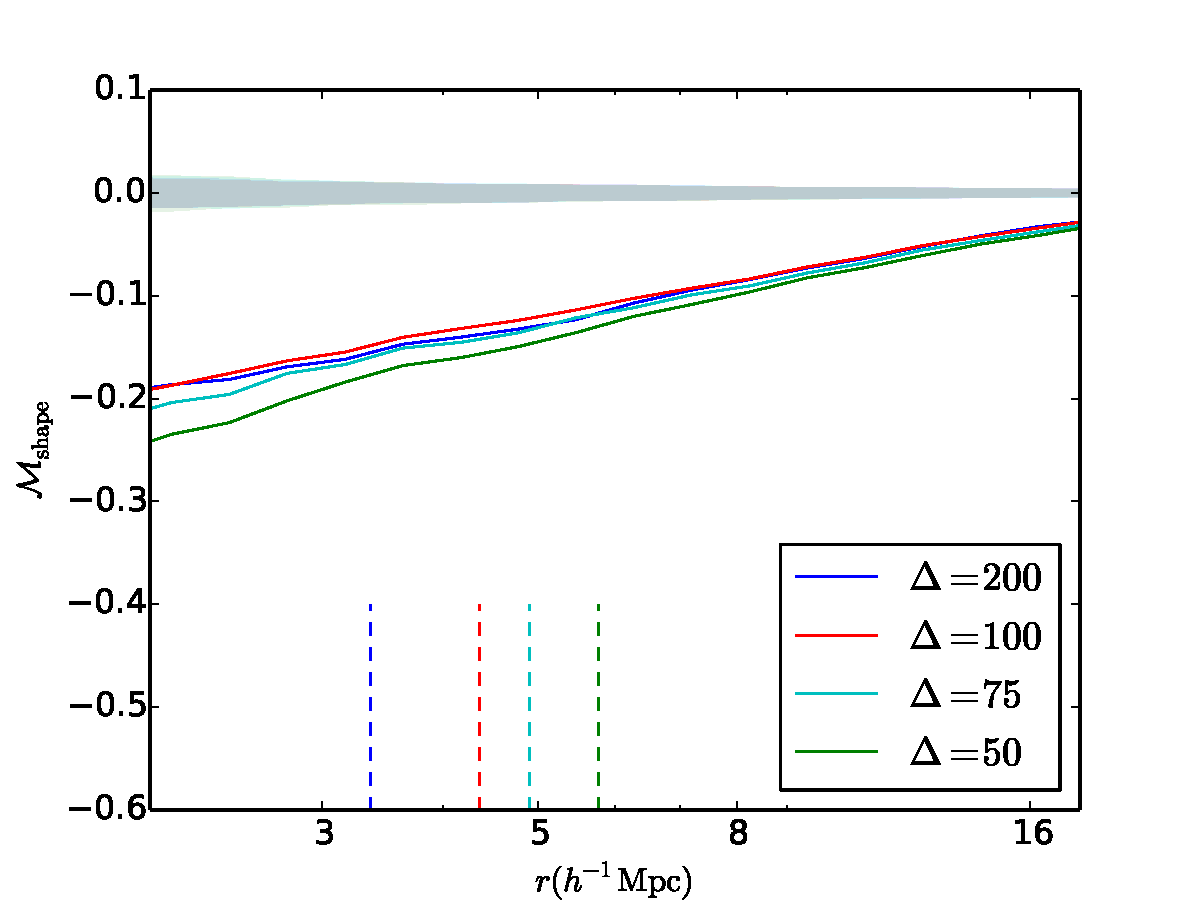
\includegraphics[width=.45\textwidth]{L0250_mcf_s_z00_l0125cut.pdf}} }
	\caption{The marked correlation function for the shape of the halo utilizing the 'l0125cut' mass cutoffs. The shaded bands represent 2-sigma confidence regions generated by randomization of the marks. The dashed line denotes the largest halo radius for a given value of the overdensity parameter.}
\end{figure*}

\begin{figure*}
	\centering
	\subfloat[L0125]{{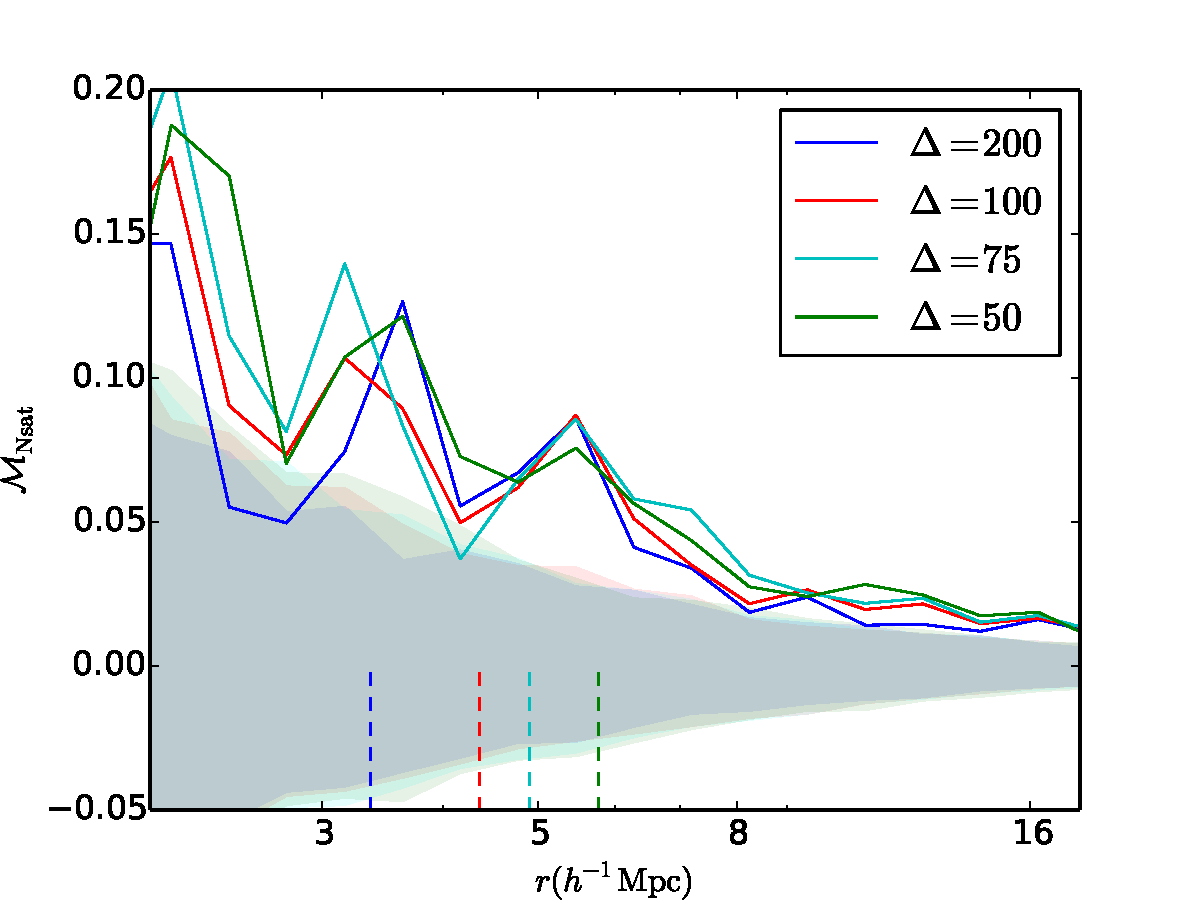
\includegraphics[width=.45\textwidth]{L0125_mcf_ns_z00_l0125cut.pdf}} }
	\subfloat[L0250]{{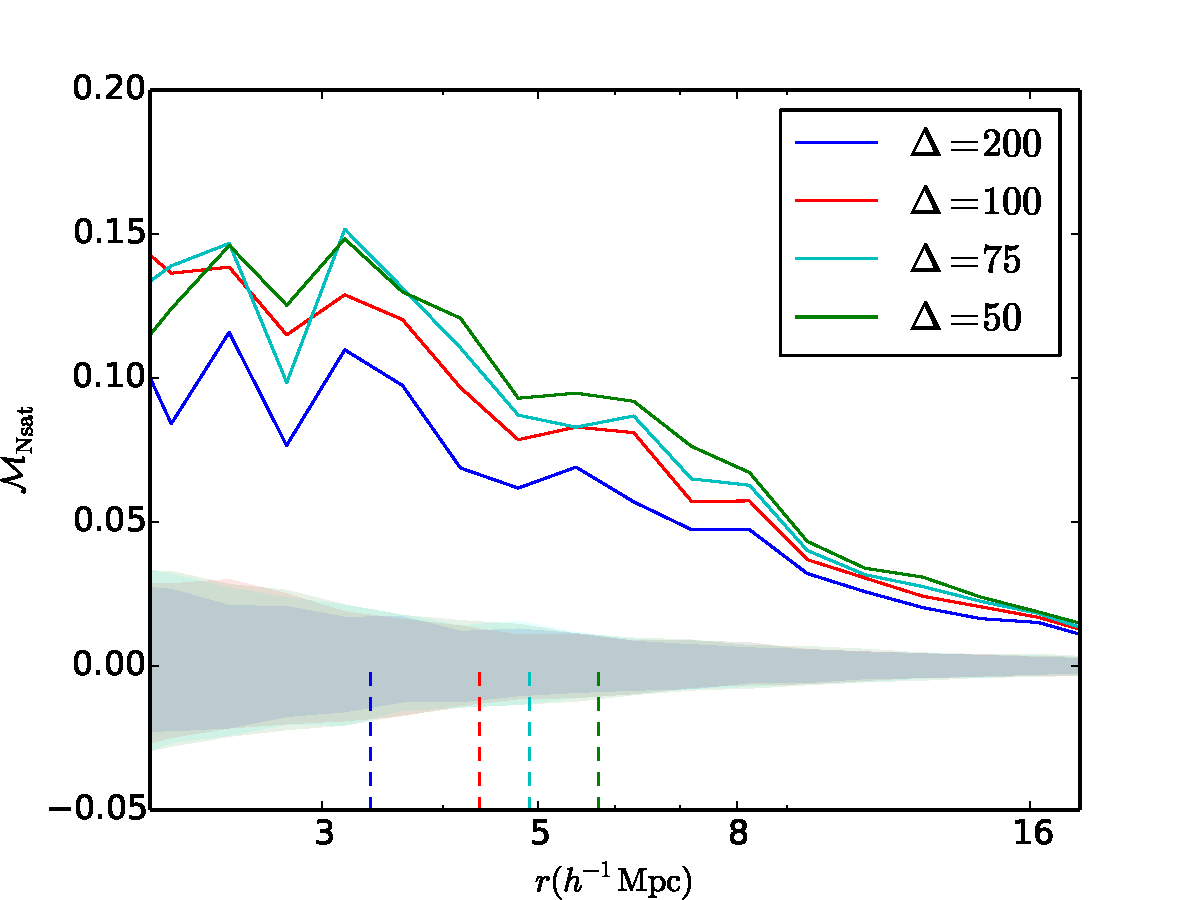
\includegraphics[width=.45\textwidth]{L0250_mcf_ns_z00_l0125cut.pdf}} }
	\caption{The marked correlation function for the satellite number utilizing the 'l0125cut' mass cutoffs. The shaded bands represent 2-sigma confidence regions generated by randomization of the marks. The dashed line denotes the largest halo radius for a given value of the overdensity parameter.}
\end{figure*}

\begin{figure*}
	\centering
	\subfloat[L0125]{{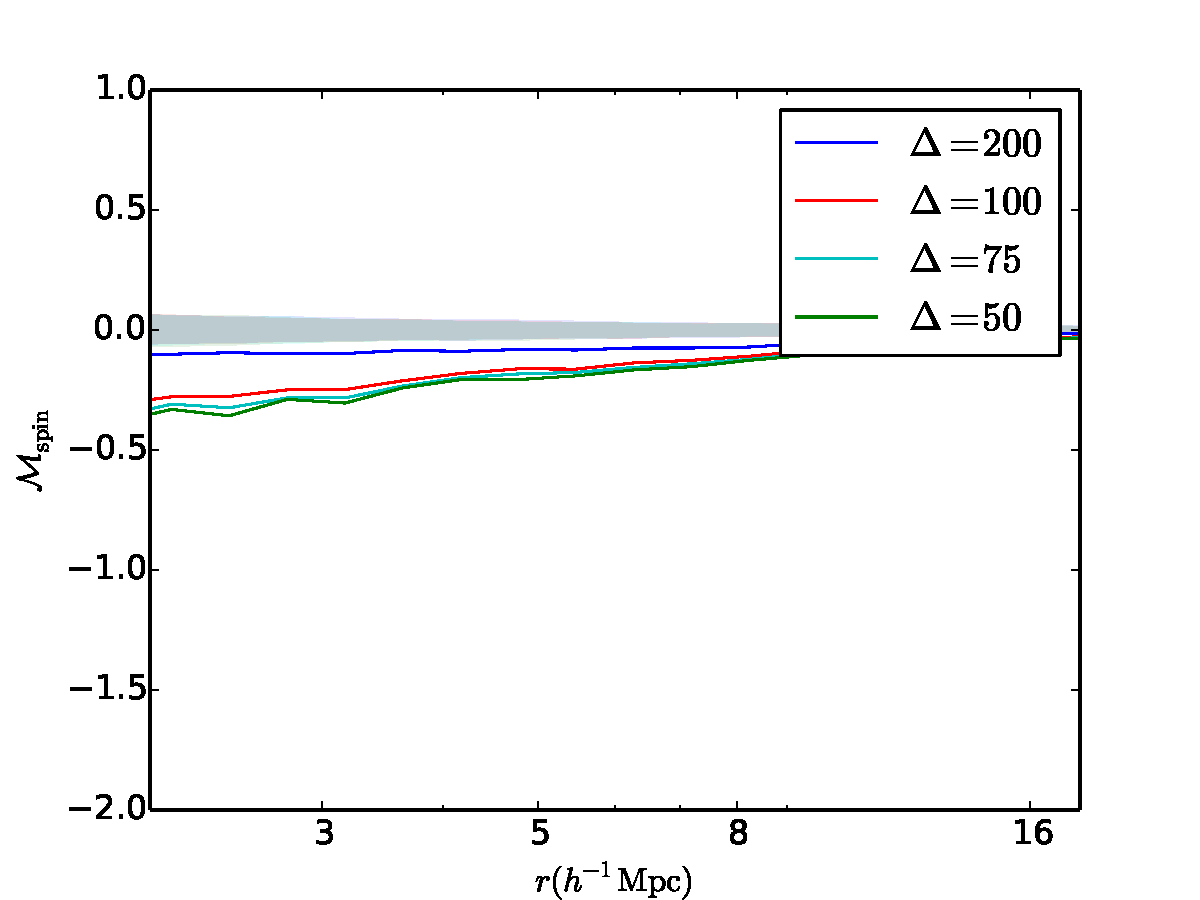
\includegraphics[width=.45\textwidth]{L0125_mcf_spin_z00_l0125cut.pdf}} }
	\subfloat[L0250]{{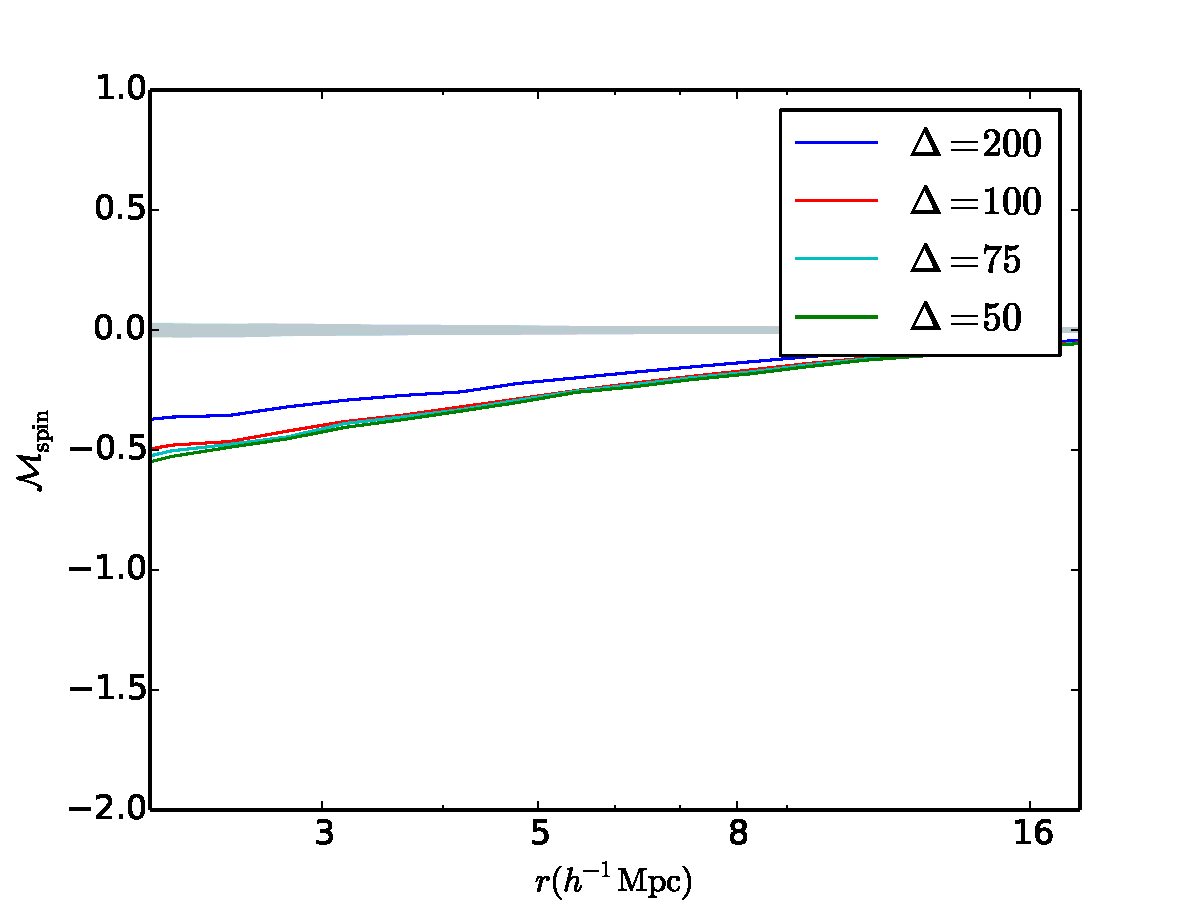
\includegraphics[width=.45\textwidth]{L0250_mcf_spin_z00_l0125cut.pdf}} }
	\caption{The marked correlation function for the spin of the halo utilizing the 'l0125cut' mass cutoffs. The shaded bands represent 2-sigma confidence regions generated by randomization of the marks. The dashed line denotes the largest halo radius for a given value of the overdensity parameter.}
\end{figure*}

% possibly remake as a single plot, though would need to be handle differently than current pipeline.

We can repeat this exercise by looking at a different set of mass cuts. In this case we will utilize our highest mass cut on the L0250 and L0500 boxes. This case does not include poorly resolved halos as we were including in the previous example. Instead, the smaller sized box runs the risk of having less of the most massive halos, resulting in having a larger variance for objects at high mass. The results of this are shown in Figures 16 through 21. There are several key observations to take away from this set of figures. It should be noted that the trend for the marked correlation functions to move is the opposite of what is seen in the low mass cut case. This seems to indicate a consistency in which you move from an excess of highly concentrated pairs in low mass bins to an excess of low concentrated pairs (or a lack of high concentrated pairs) at high mass bins. This may arise from many possible effects, though the possible exclusion due to the increased halo sizes is certainly not negligible. We also note that aside from additional noise, this trend is seen in both the L0500 and L0250 simulation boxes, asserting that this effect is not merely a statistical fluke.

\begin{figure*}
	\centering
	\subfloat[L0250]{{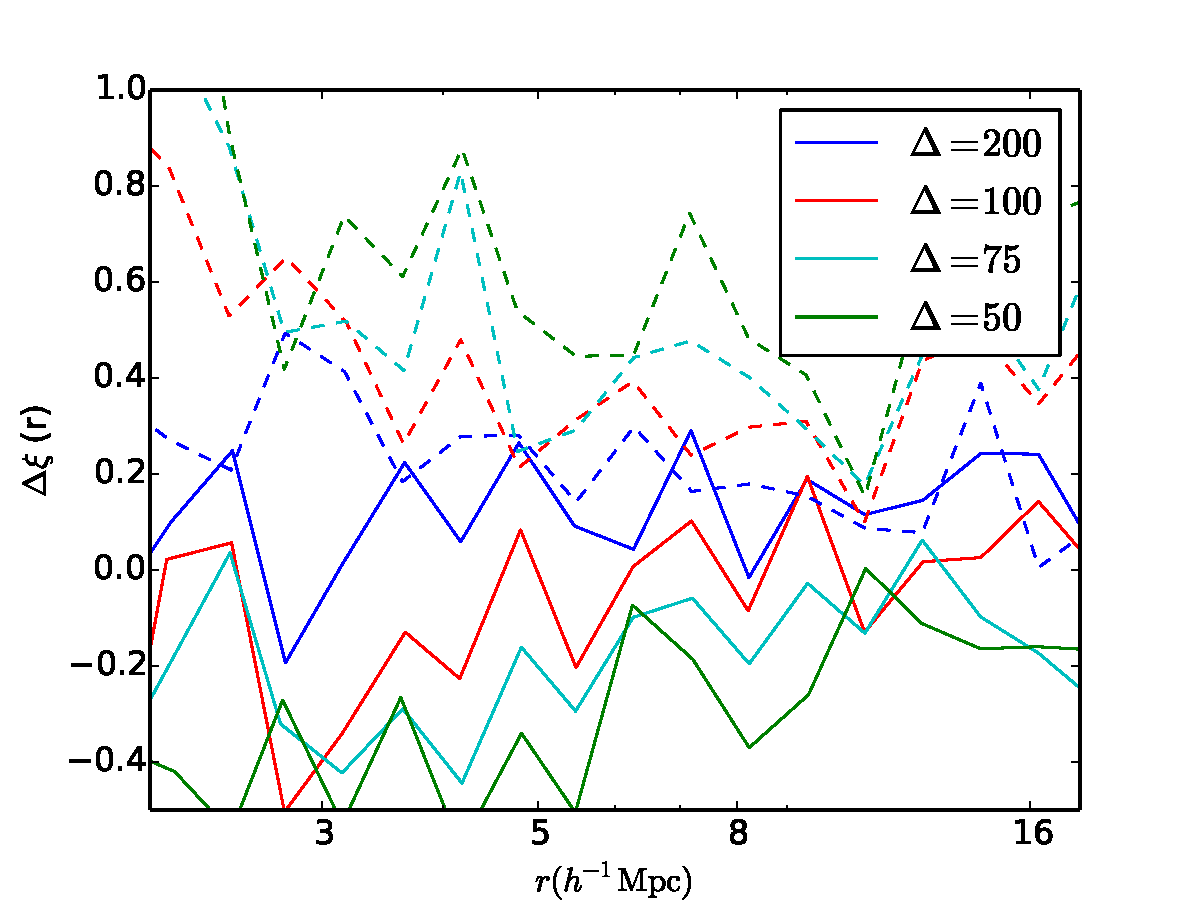
\includegraphics[width=.45\textwidth]{L0250_cf_compare_z00_l0500cut.pdf}} }
	\subfloat[L0500]{{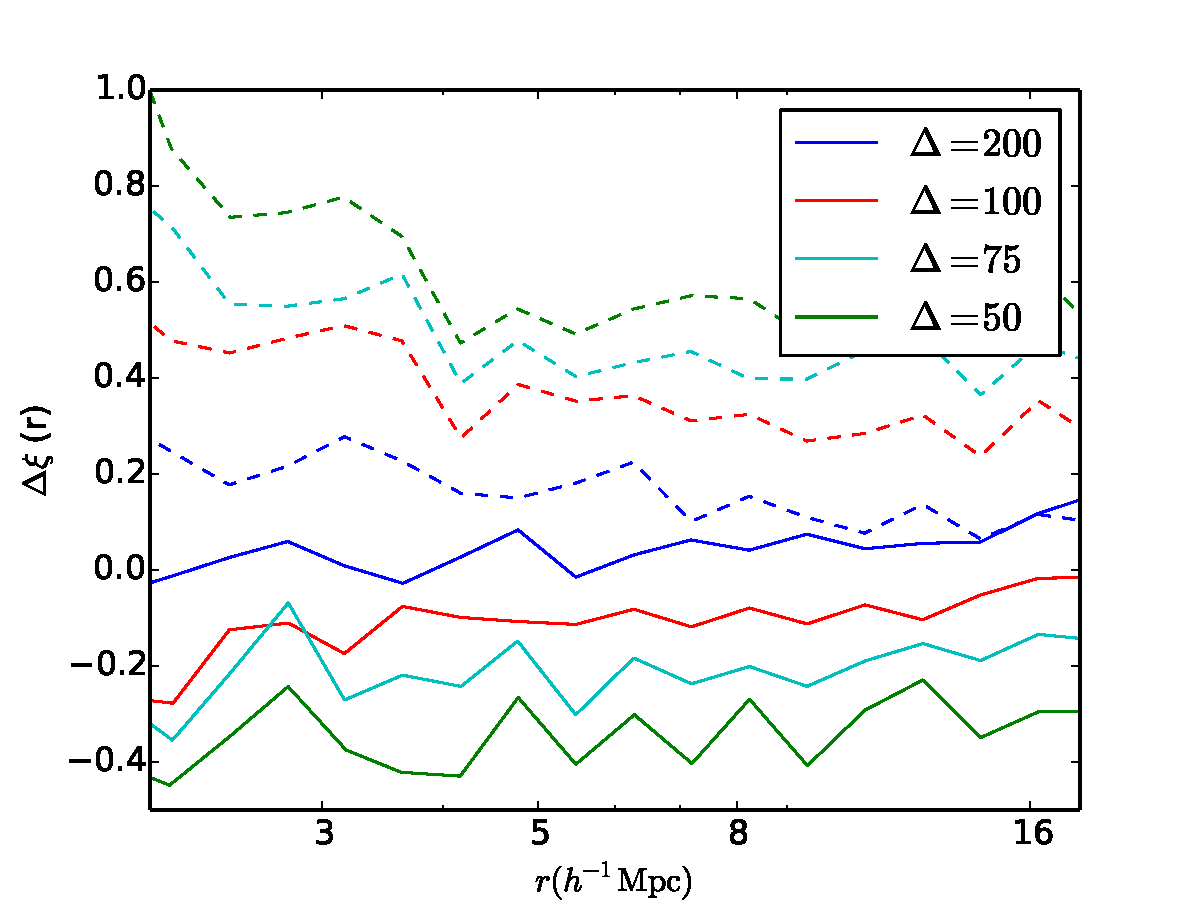
\includegraphics[width=.45\textwidth]{L0500_cf_compare_z00_l0500cut.pdf}} }
	\caption{The difference of the correlation function of all hosts compared to a cut of the 20 \% highest or lowest NFW defined concentration halos utilizing the 'l0500cut' mass cutoffs. The solid lines represent the difference from the highest concentration cut, the dashed lines represent the difference from the lowest concentration cut.}
\end{figure*}

\begin{figure*}
	\centering
	\subfloat[L0250]{{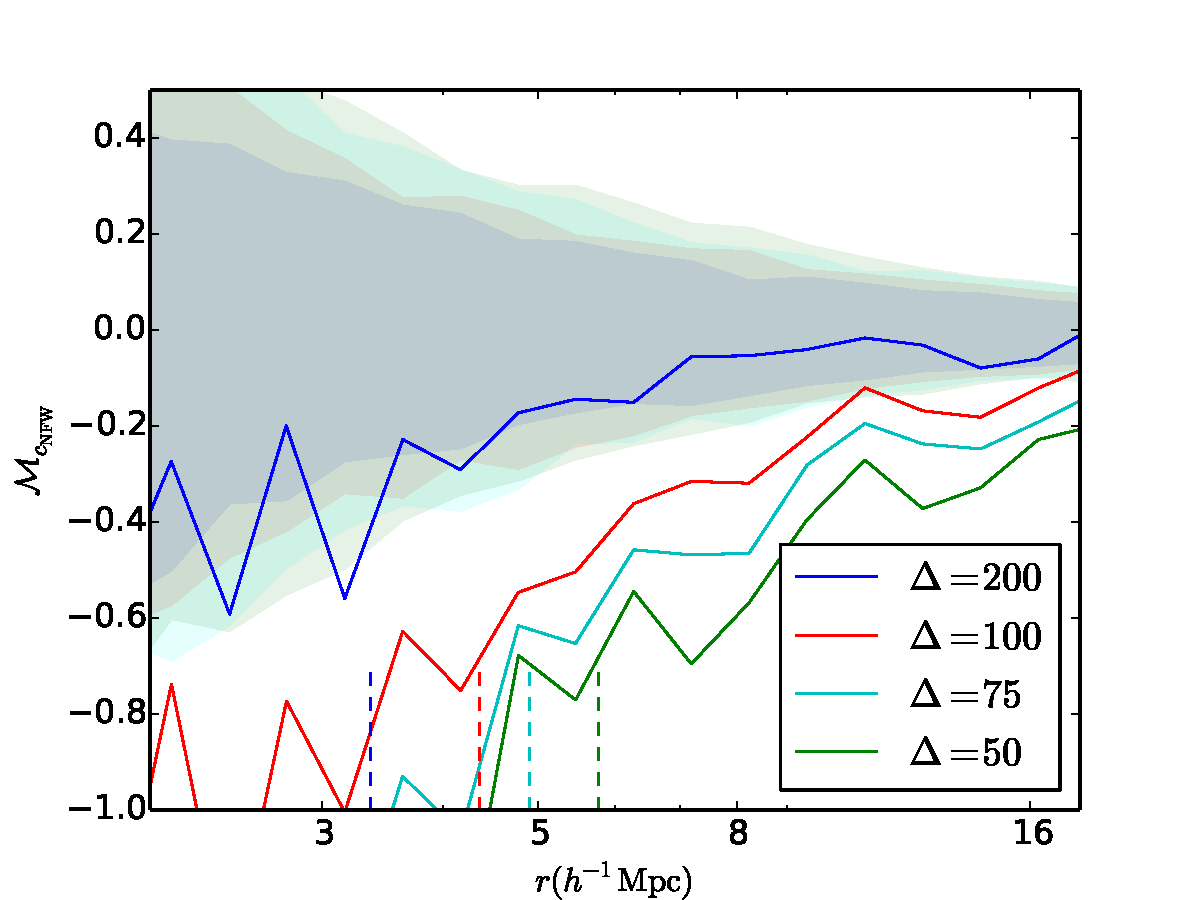
\includegraphics[width=.45\textwidth]{L0250_mcf_cnfw_z00_l0500cut.pdf}} }
	\subfloat[L0500]{{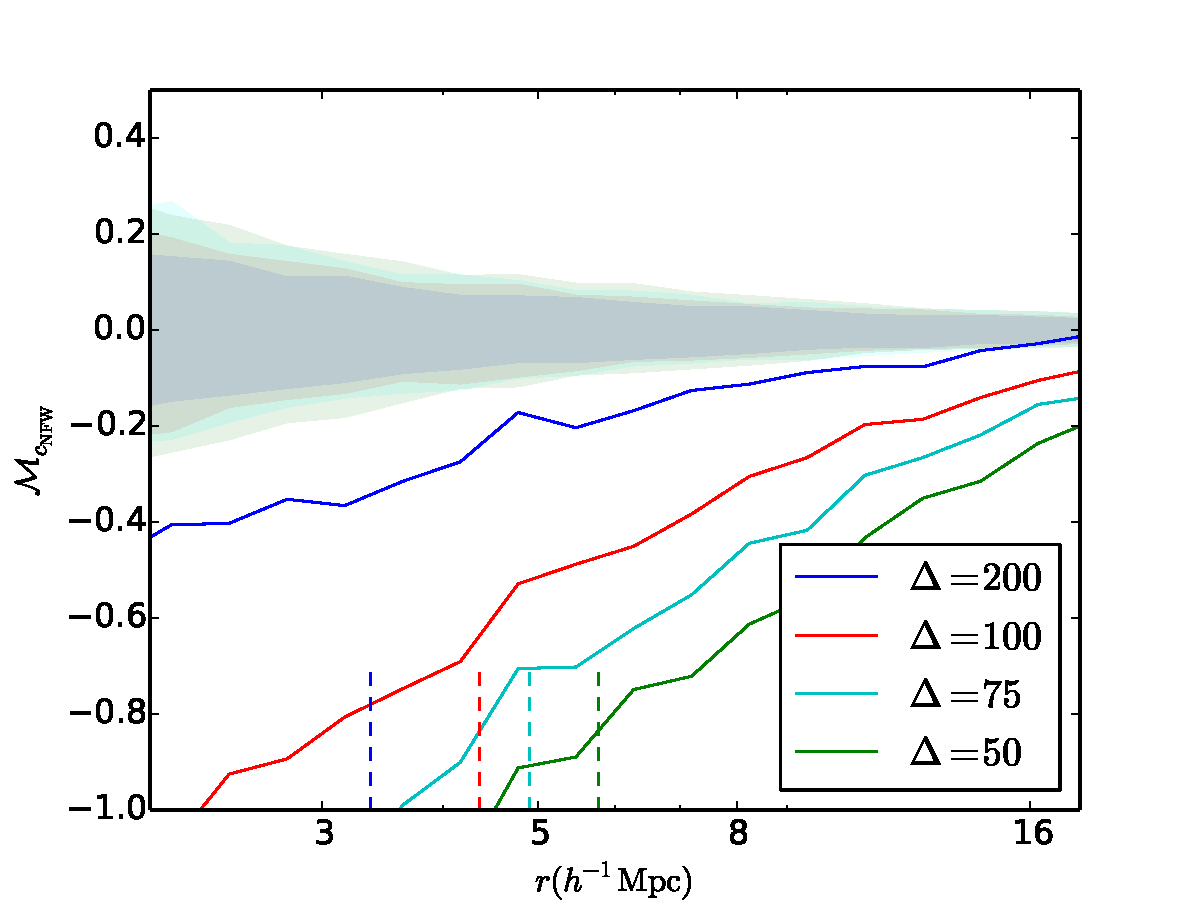
\includegraphics[width=.45\textwidth]{L0500_mcf_cnfw_z00_l0500cut.pdf}} }
	\caption{The marked correlation function for the concentration defined according to the NFW profile utilizing the 'l0500cut' mass cutoffs. The shaded bands represent 2-sigma confidence regions generated by randomization of the marks. The dashed line denotes the largest halo radius for a given value of the overdensity parameter.}
\end{figure*}

\begin{figure*}
	\centering
	\subfloat[L0250]{{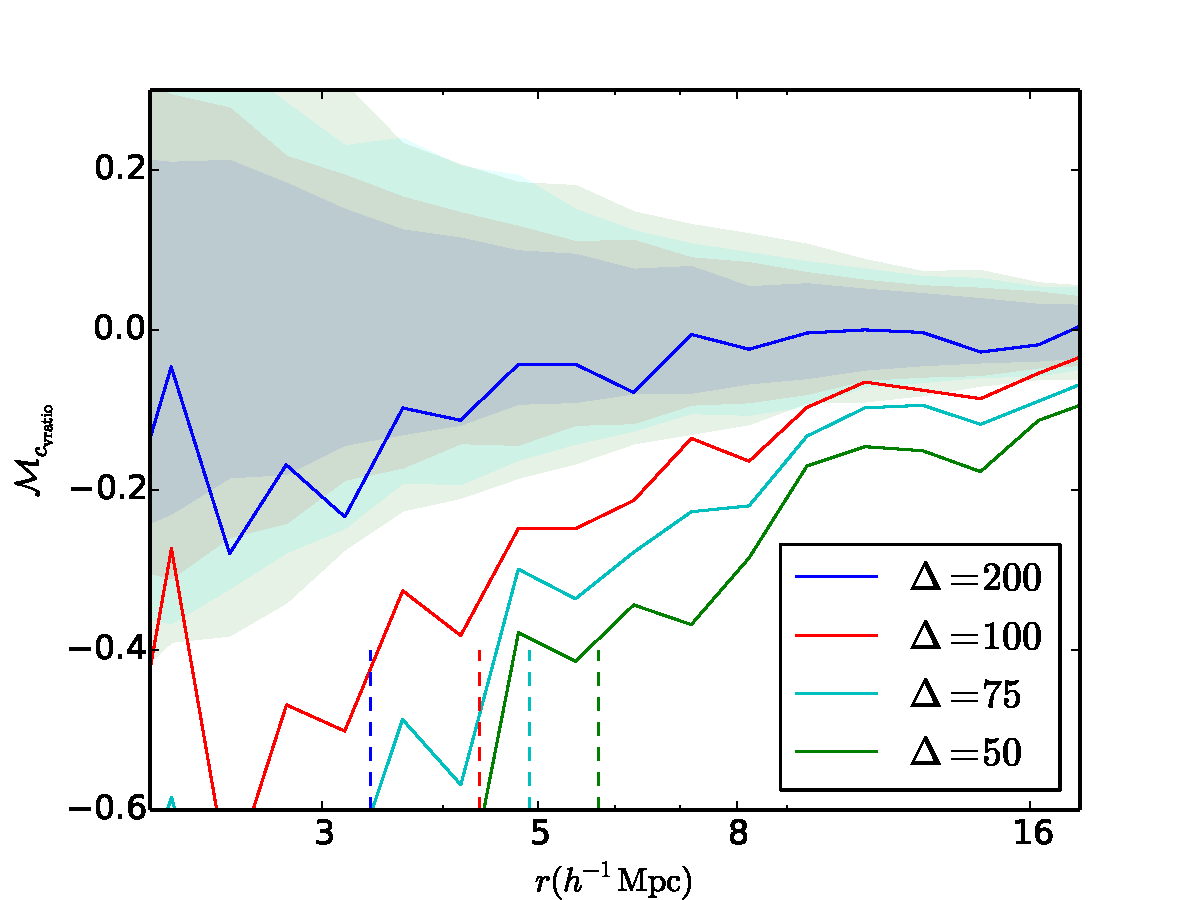
\includegraphics[width=.45\textwidth]{L0250_mcf_vrat_z00_l0500cut.pdf}} }
	\subfloat[L0500]{{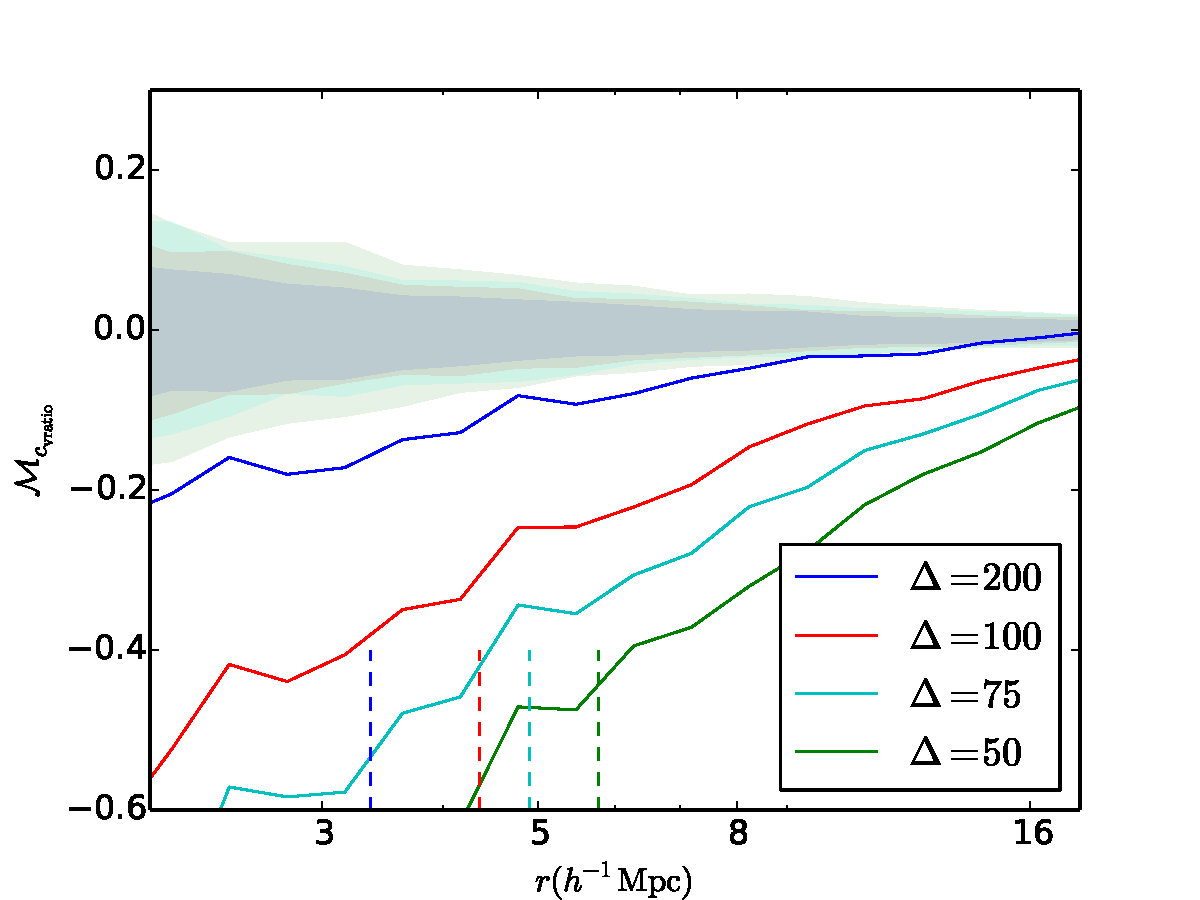
\includegraphics[width=.45\textwidth]{L0500_mcf_vrat_z00_l0500cut.pdf}} }
	\caption{The marked correlation function for the concentration defined according to the velocity ratio utilizing the 'l0500cut' mass cutoffs. The shaded bands represent 2-sigma confidence regions generated by randomization of the marks. The dashed line denotes the largest halo radius for a given value of the overdensity parameter.}
\end{figure*}

\begin{figure*}
	\centering
	\subfloat[L0250]{{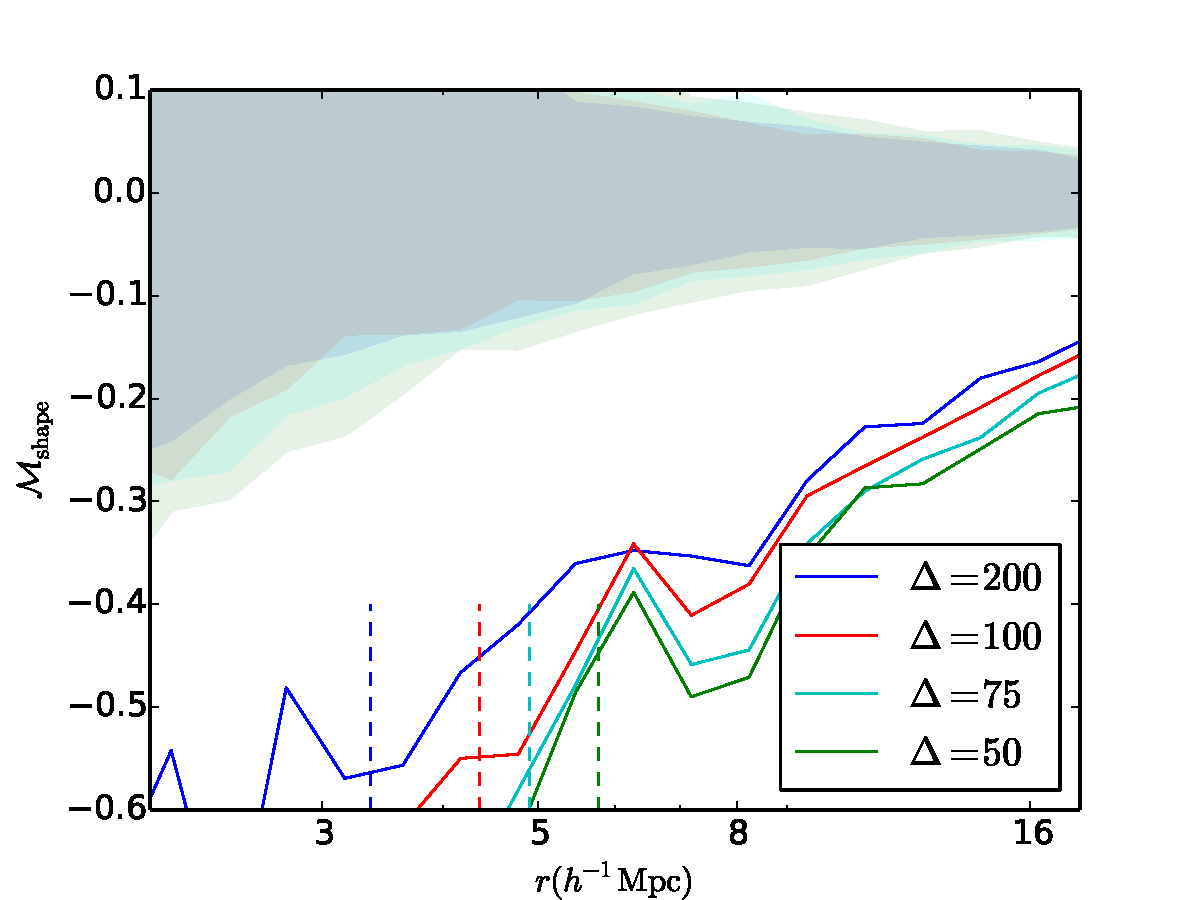
\includegraphics[width=.45\textwidth]{L0250_mcf_s_z00_l0500cut.pdf}} }
	\subfloat[L0500]{{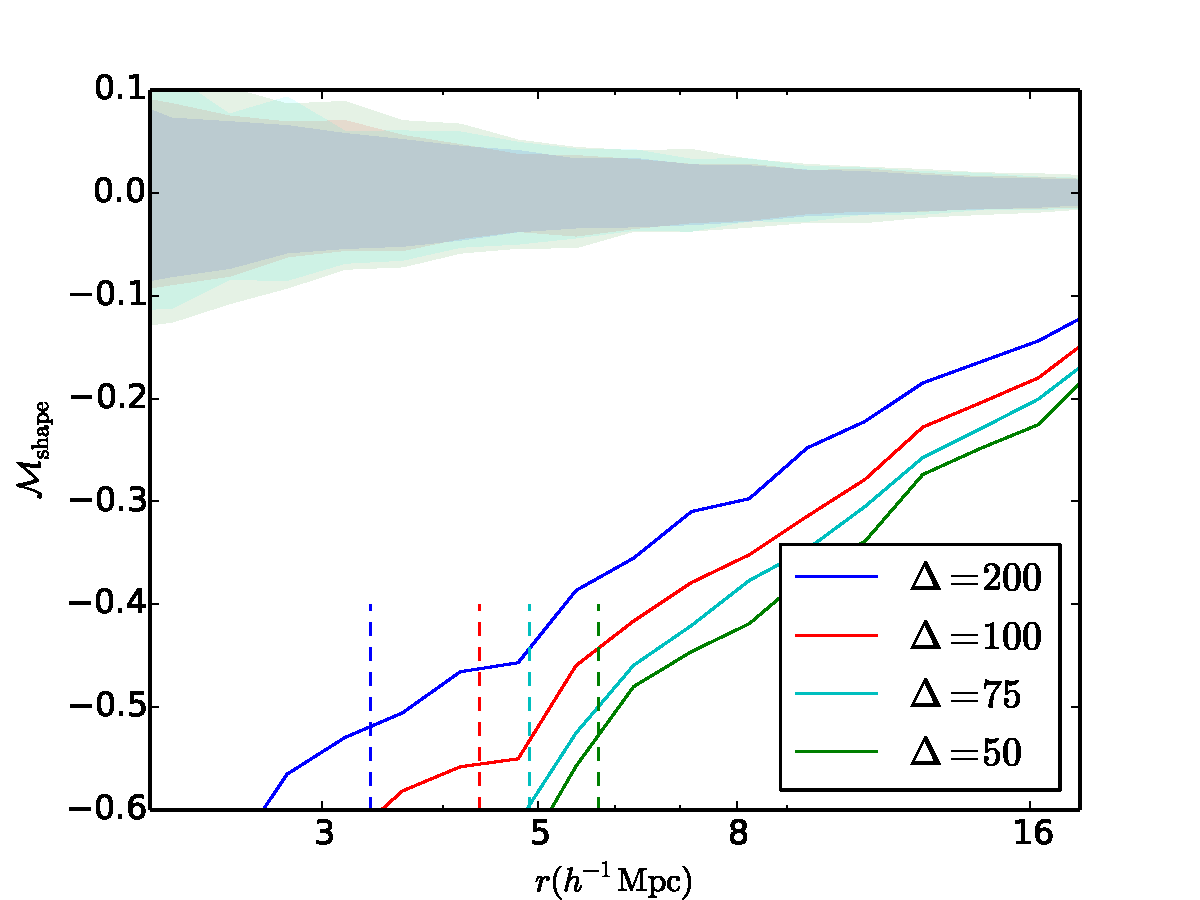
\includegraphics[width=.45\textwidth]{L0500_mcf_s_z00_l0500cut.pdf}} }
	\caption{The marked correlation function for the shape of the halo utilizing the 'l0500cut' mass cutoffs. The shaded bands represent 2-sigma confidence regions generated by randomization of the marks. The dashed line denotes the largest halo radius for a given value of the overdensity parameter.}
\end{figure*}

\begin{figure*}
	\centering
	\subfloat[L0250]{{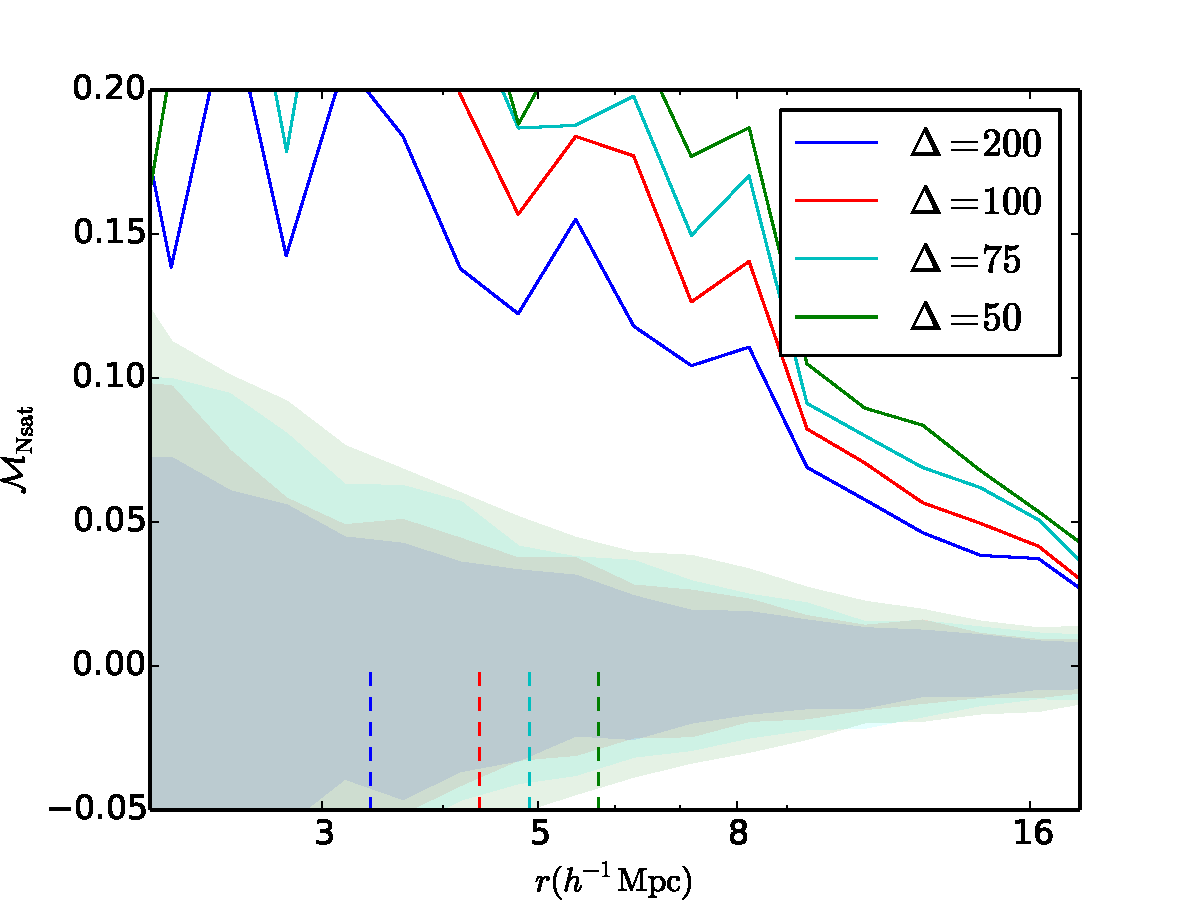
\includegraphics[width=.45\textwidth]{L0250_mcf_ns_z00_l0500cut.pdf}} }
	\subfloat[L0500]{{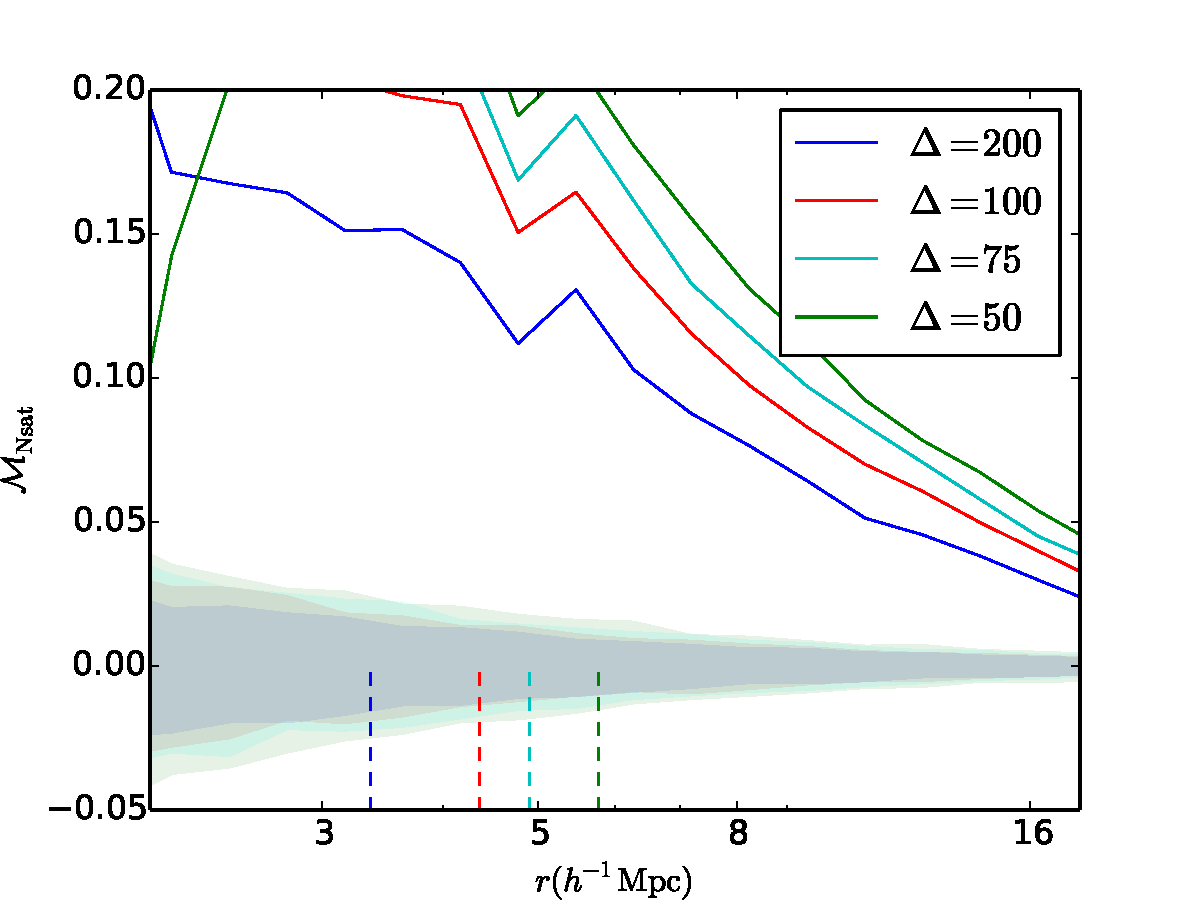
\includegraphics[width=.45\textwidth]{L0500_mcf_ns_z00_l0500cut.pdf}} }
	\caption{The marked correlation function for the satellite number utilizing the 'l0500cut' mass cutoffs. The shaded bands represent 2-sigma confidence regions generated by randomization of the marks. The dashed line denotes the largest halo radius for a given value of the overdensity parameter.}
\end{figure*}

\begin{figure*}
	\centering
	\subfloat[L0250]{{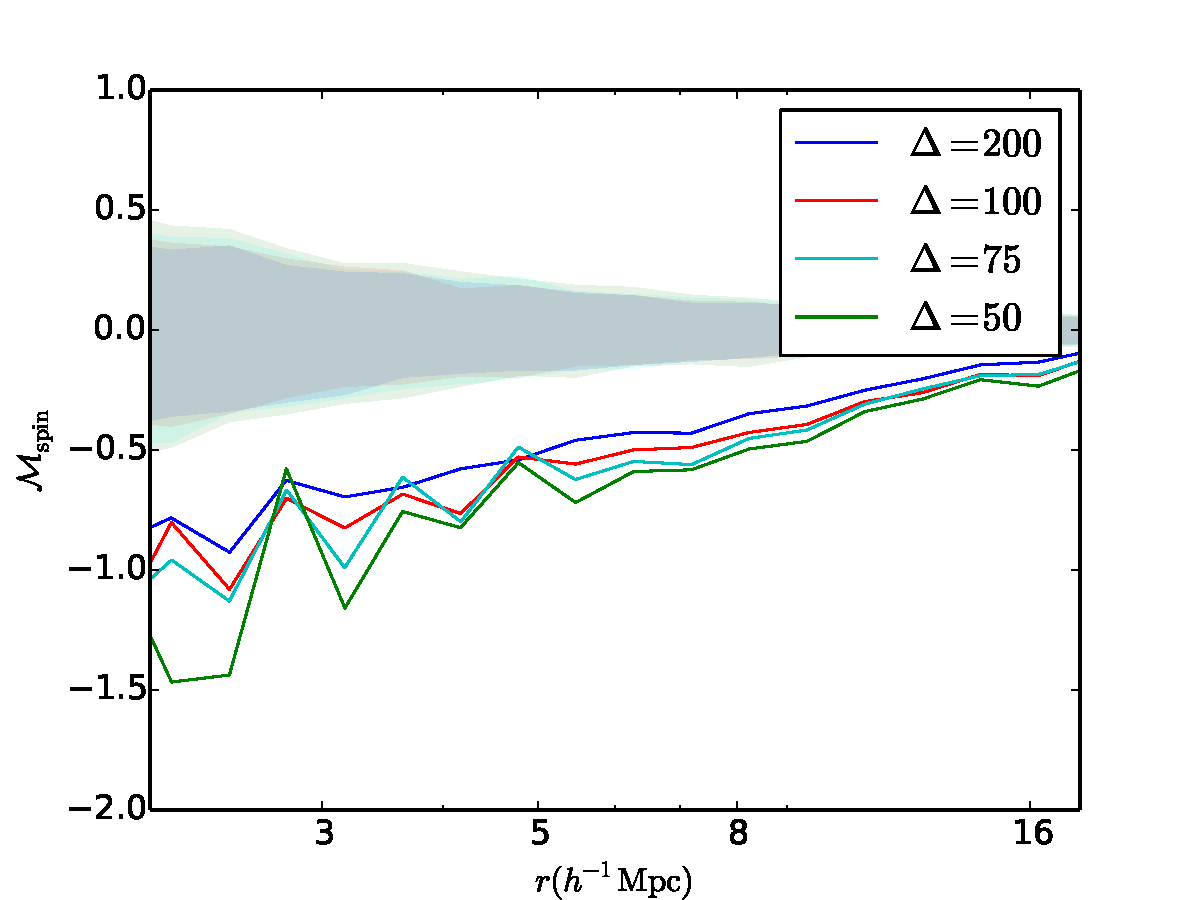
\includegraphics[width=.45\textwidth]{L0250_mcf_spin_z00_l0500cut.pdf}} }
	\subfloat[L0500]{{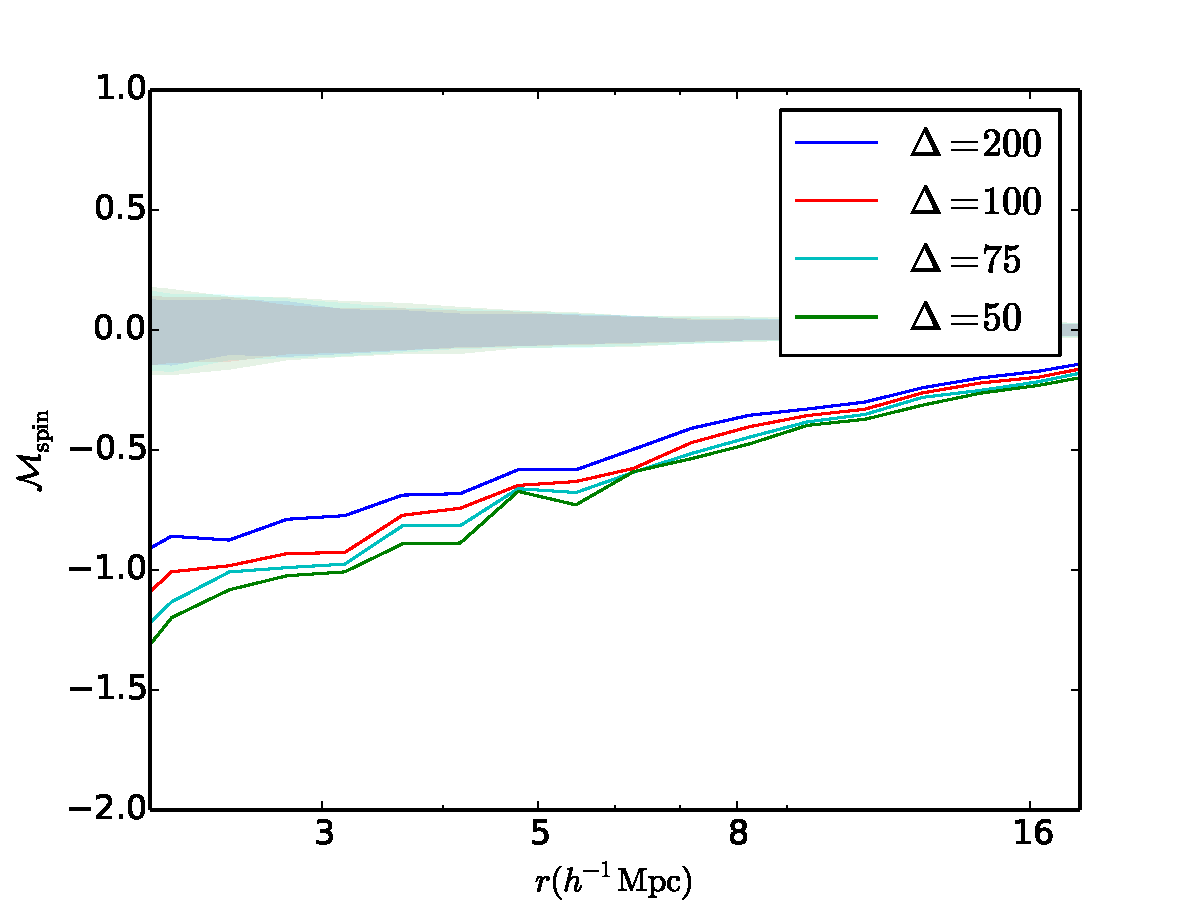
\includegraphics[width=.45\textwidth]{L0500_mcf_spin_z00_l0500cut.pdf}} }
	\caption{The marked correlation function for the spin of the halo utilizing the 'l0500cut' mass cutoffs. The shaded bands represent 2-sigma confidence regions generated by randomization of the marks. The dashed line denotes the largest halo radius for a given value of the overdensity parameter.}
\end{figure*}



%----------------------
\section[]{Conclusions}
\label{section:conclusions}
%----------------------

We have looked at how to use CFs and MCFs in order to analyze the environmental effects upon the properties of the halo. We have suggested a method of removing the mass dependence that is not subject to the small number statistics at large halo masses. Taking our various tests, we then apply a change to the threshold density $\Delta$ in an attempt to remove the effect that environment has upon these properties. We come to the following conclusions from our simulation data.

\begin{itemize}
	\item Our halo redefinition method does not cause any substantial breakdown in the ROCKSTAR halo finding algorithm, though this may not be the case for every halo finding methodology. This is something that should be considered prior to utilization of this method, unless working directly from particle data. As our initial halo sizes and locations are determined through spherical overdensities, it cannot be assumed that starting from a FoF grouping and then determining values through particle data directly will produce identical results. Similarly, different cosmologies may remove environmental effects at different scales.

	\item When looking at the two-point correlation function, there appears to be a ``sweet spot'' that appears to remove environmental effects the most efficiently. Going beyond that seems to reintroduce environmental effects, possibly as an extreme side effect of halo exclusion.

	\item For our marked correlation functions we see that both proxies of concentration that we use as marks show significant removal of environmental effects at large scales for similar values of the overdensity parameter $\Delta$. In cases where one is only interested in the concentration of dark matter halos and large scales (or correspondingly small values of k), this method will allow you to compensate for bias that environment could introduce to calculations dependent upon the halo model. This may prove valuable for calculations such as that of the shear power spectrum calculated through weak lensing.

	\item The environmental effects on the shape of the host halo and the satellite number of the host halo cannot be removed regardless of the chosen redefinition of $\Delta$. We propose that this may be intrinsically tied to the nature of the filaments, whose effects cannot be removed by a simple redefinition of the halo radius.

	\item This method is definitively related to the mass of the halos that are being observed. Furthermore, it appears that the majority of the reduction in assembly bias is tied to the exclusion of halos from the catalog as a result of being subsumed into larger halos. This information does not seem to be contradictory; it can be intuitively understood that the region about the most massive halos will be different than the region around the least massive halos, leading to a different frequency at which halos are being excluded. It does however warrant that careful consideration be given to the sample of halos that are of interest.
\end{itemize}

This methodology, while certainly not perfect in removing environmental effects, may be of significance when applied to galaxy formation models. Provided that the properties of interest in a given model behave well under our redefinition, it will allow us to create better mock galaxy catalogs while avoiding the trouble that baryonic physics represent. This may allow us to better study the properties of galaxies within halos without having to substantially increase computation time. There remain possible uncertainties to study in the future. 

\section*{Acknowledgments}

We are grateful to many people.

%%\bibliographystyle{plainnat}
\bibliography{master}

\label{lastpage}

\end{document}
